\documentclass[10pt]{article}
\renewcommand{\baselinestretch}{1.8}

\usepackage[b4paper,left=0.8in,right=0.8in,top=0.8in,bottom=0.8in]{geometry}
\usepackage{tikz-qtree}
\usepackage{algorithm}
\usepackage{algpseudocode}
\makeatletter
\renewcommand{\ALG@beginalgorithmic}{\footnotesize}
\makeatother
\usepackage{graphicx}
\usepackage{subcaption}
\usepackage{showkeys}
\usepackage{amsmath}


\usepackage{multicol}
\setlength\columnsep{24pt}

\algnewcommand\algorithmicforeach{\textbf{for each}}
\algdef{S}[FOR]{ForEach}[1]{\algorithmicforeach\ #1\ \algorithmicdo}

\algdef{S}[FUNCTION]{Function}
   [3]{{\texttt{\textsl{#1}}} \textproc{\texttt{#2}}\ifthenelse{\equal{#3}{}}{}{\texttt{(#3)}}}
  
\algdef{E}[FUNCTION]{EndFunction}
   [1]{\algorithmicend\ \texttt{\textproc{#1}}}

\algrenewcommand\Call[2]{\texttt{\textproc{#1}\ifthenelse{\equal{#2}{}}{}{(#2)}}}
   
\newcommand\keywordfont{\sffamily\bfseries}
\algrenewcommand\algorithmicend{{\keywordfont end}}
\algrenewcommand\algorithmicfor{{\keywordfont for}}
\algrenewcommand\algorithmicforeach{{\keywordfont for each}}
\algrenewcommand\algorithmicdo{{\keywordfont do}}
\algrenewcommand\algorithmicuntil{{\keywordfont until}}
\algrenewcommand\algorithmicfunction{{\keywordfont function}}
\algrenewcommand\algorithmicif{{\keywordfont if}}
\algrenewcommand\algorithmicthen{{\keywordfont then}}
\algrenewcommand\algorithmicelse{{\keywordfont else}}
\algrenewcommand\algorithmicreturn{{\keywordfont return}}

\renewcommand\thealgorithm{}
\newcommand{\setalglineno}[1]{%
  \setcounter{ALC@line}{\numexpr#1-1}}


\title{Wait-free Queues with Polygarithmic Step Complexity}
\date{\today}

\usepackage{amsmath,amssymb,amsthm}
\newtheorem{theorem}{Theorem}
\newtheorem{lemma}[theorem]{Lemma}
\theoremstyle{definition}
\newtheorem{definition}[theorem]{Definition}

\begin{document}
\maketitle

%\begin{abstract}
%This is the paper's abstract \ldots
%\end{abstract}

\section{Previous Work}
\begin{table}[hbt]
  \begin{center}
  \begin{tabular}{l|c|c|c}
    & Type & Progress Property  & Complexity \\ \hline
    MichaelS96~\cite{DBLP:conf/podc/MichaelS96} & Singly Linked List & Lock-free & $\Omega(p)$ \\ \hline
    MoirNSS05~\cite{DBLP:conf/spaa/MoirNSS05} & Linked List with Elemination & & \\ \hline
    HoffmanSS07~\cite{DBLP:conf/opodis/HoffmanSS07} & Linked List with Baskets & & $\Omega(p)$ \\ \hline
    Ladan-MozesS08 ~\cite{DBLP:journals/dc/Ladan-MozesS08} & Doubly linked list & Lock-free & $\Omega(p)$ \\ \hline
    MilmanKLLP18~\cite{DBLP:conf/spaa/MilmanKLLP18} & Linked List with batching same type ops & Lock-free & \\ \hline
    GidenstamST10~\cite{DBLP:conf/opodis/GidenstamST10} & Linked list of arrays & Lock-free & $\Omega(p+len(array))$ \\ \hline
    KoganP11~\cite{DBLP:conf/ppopp/KoganP11} &  Linkedlist with head and tail pointers & Wait-free & $\textsc{O}(p\times\text{bakery-max})$
  \end{tabular}
  \caption{Linearizable ME-MD Queus}
  \end{center}
\end{table}

\section{ Universal Construction using Tournament Tree with Big CAS Objects }
\paragraph{}
Jayanti~\cite{DBLP:conf/podc/Jayanti98a} proved an $\Omega(\log p)$ lower bound on the worst-case shared-access time complexity of $p$-process universal constructions. He also introduced~\cite{DBLP:conf/podc/ChandraJT98} a construction that achieves $\textsc{O}(\log^2 p)$ shared accesses. Here, we first introduce a universal construction using $\textsc{O}(\log p)$ CAS operations~\cite{DBLP:conf/fsttcs/JayantiP05}. We use the universal construction as a stepping stone towards our queue algorithm, so we will not explain it in too much detail.
\paragraph{}
We introduce our universal construction in Algorithm~\ref{alg1} with a tournament tree with $p$ leaves and height $\log(p)$ is shared among $p$ processes. Nodes are CAS objects, and each leaf is assigned to one process exclusively. Each CAS object stores a sequence of operations. When process $P_i$ wishes to apply an operation $op$ on the implemented object, it appends $op$ to its assigned leaf and tries to propagate it up to the root. The sequence of operations stored in Node $n$'s CAS object shows the order of the operations propagated up to $n$.
The history of operations stored at the root is the linearization ordering. The operation $op$ is linearized when it is appended to the root.

\begin{center}
\Tree [ [ [ $P_1$ $P_2$ ] [ $P_3$ $P_4$ ] ]
          [ [ $P_5$ $P_6$ ] [ $P_7$ $P_8$ ] ] ]
\end{center}


Leaf $l_i$ stores the sequence of the operations invoked by $P_i$. 
The algorithm uses a subroutine \textsc{Refresh}($n$) that concatenates new operations from node $n$'s children (that have not already been propagated to $n$) to the sequence of operations stored in $n$ and tries to CAS the new sequence into $n$. In other words, \textsc{Refresh}($n$) tries to append $n$'s children's new operations to $n$'s sequence.
After a process adding a new operations to its leaf, it has to propagate new operations up to the root. \textsc{Propagate}($n$) tries to append $n$'s new operations to the root $n$ by recursively calling \textsc{Refresh}($n$). In each step if a \textsc{Refresh}($n$) fails, it means another CAS operation has succeeded; if so, it tries to \textsc{Refresh}($n$) again. If the second attempt fails too, another process has already appended the operations the current \textsc{Propagate} is trying to append.
Operations that were in $l_i$ before \textsc{Propagate}($l_i$.parent) was invoked are guaranteed to be added to the root by the time the \textsc{Propagate}($l_i$.parent) finishes.



\begin{figure}

\begin{center}


\begin{subfigure}[b]{.49\textwidth}


  \centering
  \resizebox{\columnwidth}{!}{
  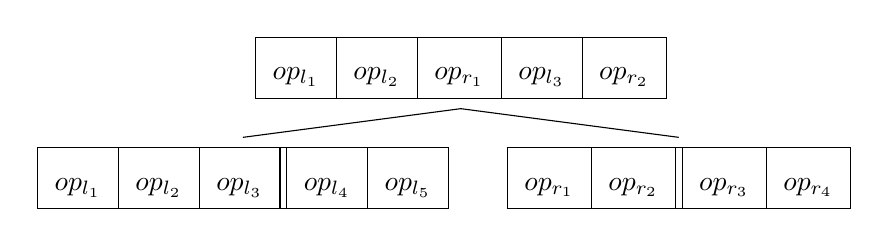
\begin{tikzpicture}[level 1/.style={level distance=1.4cm,sibling distance=0.5cm}]
\Tree [.{\begin{tabular}{|c|c|c|c|c|c|}  \hline $op_{l_1}$ & $op_{l_2}$ & $op_{r_1}$ & $op_{l_3}$ & $op_{r_2}$ \\ \hline \end{tabular}}
{\begin{tabular}{|c|c|c||c|c|}  \hline $op_{l_1}$ & $op_{l_2}$ & $op_{l_3}$ & $op_{l_4}$ & $op_{l_5}$ \\ \hline \end{tabular}}
{\begin{tabular}{|c|c||c|c|}  \hline $op_{r_1}$ & $op_{r_2}$ & $op_{r_3}$ & $op_{r_4}$\\ \hline \end{tabular}} ]
\end{tikzpicture}
}
  \caption{Operations after $||$ are new.}

\end{subfigure}
\hfill
\begin{subfigure}[b]{.49\textwidth}


  \centering
  \resizebox{\columnwidth}{!}{
  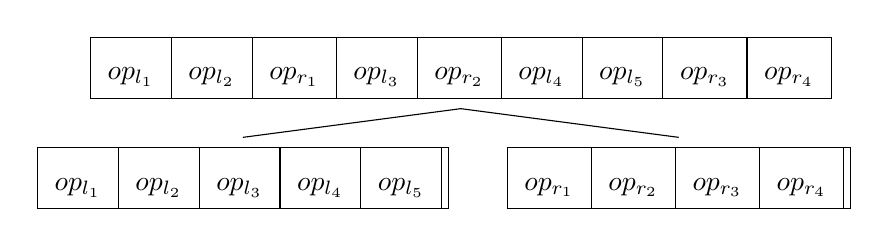
\begin{tikzpicture}[level 1/.style={level distance=1.4cm,sibling distance=0.5cm}]
\Tree [.{\begin{tabular}{|c|c|c|c|c|c|c|c|c|c|}  \hline $op_{l_1}$ & $op_{l_2}$ & $op_{r_1}$ & $op_{l_3}$ & $op_{r_2}$ & $op_{l_4}$ & $op_{l_5}$ & $op_{r_3}$ & $op_{r_4}$  \\ \hline \end{tabular}}
{\begin{tabular}{|c|c|c|c|c||}  \hline $op_{l_1}$ & $op_{l_2}$ & $op_{l_3}$ & $op_{l_4}$ & $op_{l_5}$ \\ \hline \end{tabular}}
{\begin{tabular}{|c|c|c|c||}  \hline $op_{r_1}$ & $op_{r_2}$ & $op_{r_3}$ & $op_{r_4}$\\ \hline \end{tabular}} ]
\end{tikzpicture}
}
  \caption{New operations are added to the parent node.}

\end{subfigure}


\caption{\label{fig:ucexample} Propagate Step in Universal Construction}
\end{center}
\end{figure}


\begin{algorithm}
\caption{Universal Construction Idea}\label{alg1}
\begin{algorithmic}[1]
\begin{multicols}{2}

\Function{response}{Do}{\textsl{operation} op, \textsl{pid} i} 
\State \texttt{l\textsubscript{i}.\Call{append}{op}}
\State \Call{Propagate}{parent of l\textsubscript{i}}
\State \texttt{Run} \textsf{the sequence stored in root}
\State \texttt{\Return op}\textsf{'s response from line 4}
\EndFunction{Do}

\Statex

\Function{void}{Propagate}{\textsl{node} n}
\If{\texttt{n==root}} \Return
\ElsIf{!\Call{Refresh}{n}}
\State \Call{Refresh}{$n$} \EndIf
\State \Call{Propagate}{parent of n}
\EndFunction{Propagate}

\columnbreak

\Function{boolean}{Refresh}{\textsl{node} n}
\State \texttt{old=} \Call{Read}{n}
\State \texttt{new=} \textsf{ops that n's children contain but \texttt{old} does not}
\State \texttt{new= old$\cdot$new}
\State \Return n.\Call{CAS}{old, new}
\EndFunction{Refresh}

\end{multicols}
\end{algorithmic}
\end{algorithm}

$\textsc{O}(\log n)$ CAS operations are invoked to do a \textsc{Propagate}, but the CAS words store sequences of unbounded length.
The problem is that we are trying to store unbounded sequence of operations in each node $n$ (see Figure~\ref{fig::uc}). However, to compute the result of an operation, we only use the total ordering that is stored at the root. Although we use a similar construction for our queue implementation, we develop an implicit representation of the sequence of operations, so that we can use reasonable size CAS objects and still achieve polygarithmic step complexity.

\begin{figure}[h]
\begin{center}
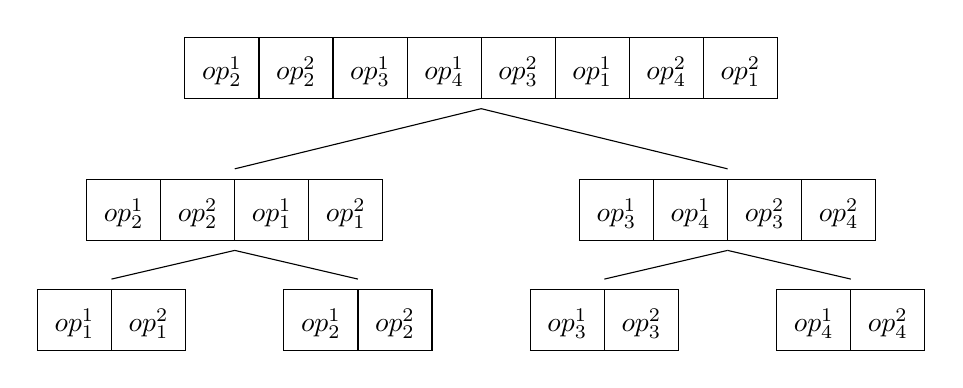
\begin{tikzpicture}[level 1/.style={level distance=1.8cm,sibling distance=1cm}, level 2/.style={level distance=1.4cm,sibling distance=1cm}]
  
\Tree [.{\begin{tabular}{|c|c|c|c|c|c|c|c|c|c}  \hline  $op_2^1$ & $op_2^2$ & $op_3^1$ & $op_4^1$ & $op_3^2$ & $op_1^1$ & $op_4^2$ & $op_1^2$ \\ \hline\end{tabular}}  [.{\begin{tabular}{|c|c|c|c|c|c}  \hline $op_2^1$ & $op_2^2$ & $op_1^1$ & $op_1^2$ \\ \hline\end{tabular}}
      {\begin{tabular}{|c|c|c|c}  \hline $op_1^1$ & $op_1^2$ \\ \hline\end{tabular}} {\begin{tabular}{|c|c|c|c}  \hline $op_2^1$ & $op_2^2$ \\ \hline\end{tabular}} ] [.{\begin{tabular}{|c|c|c|c|c|c}  \hline $op_3^1$ & $op_4^1$ & $op_3^2$ & $op_4^2$ \\ \hline\end{tabular}} {\begin{tabular}{|c|c|c|c}  \hline $op_3^1$ & $op_3^2$ \\ \hline\end{tabular}} {\begin{tabular}{|c|c|c|c}  \hline $op_4^1$ & $op_4^2$ \\ \hline\end{tabular}} ] ]

\end{tikzpicture}
\caption{\label{fig::uc} Universal Construction: $op_j^i$ denotes the $i$th operation from process $j$. In each node, we store the ordering of all the operations propagated up to it.}
\end{center}
\end{figure}

\section{Block Tree}

%\subsection{Idea in a nutshell}
We apply two ideas from universal construction to create a new linearizable data structure agreeing on a sequence of elements among processes. First, there is a shared tournament tree among processes, in which each process appends its element to its leaf in the tree and then tries to propagate it up to the root by performing \textsc{Refresh()} operations at each node. Second, each operation is linearized when its element is appended to the root.

\subsection{Sequence of propagated operations}
\paragraph{}
The basic idea behind the universal construction is to create a linearization of operations invoked by processes. If we design a fast shared data structure in which processes can append elements to a sequence, we can use it to implement practical, fast implementaion of an object $O$ by using the sequence data structure to keep track of the sequence of operations  on $O$. In the following sections, we introduce our solution called Block~Tree.

%\begin{lemma}
%    Consider an instance of \textsc{Propagate(}\textnormal{n}\textsc{)}. When it terminates all operations that were in $n$ before \textsc{Propagate(}\textnormal{n}\textsc{)} will be in the root. \texttt{(not suitable place)}
%\end{lemma}

\subsection{Sequence of Sets of Concurrent Operations \label{subsec::block}}
\paragraph{}
 In the universal construction, we order new concurrent operations at each \textsc{Refresh}() and maintain that order in the path up to the root. However, we can instead keep track of sets of concurrent operations and create the total ordering of all operations at the root (see Figure~\ref{fig::set}).
 
 \begin{figure}[h]
\begin{center}
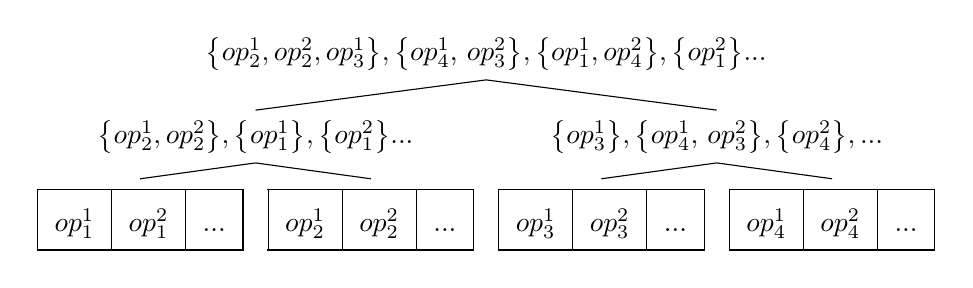
\begin{tikzpicture}
  
\Tree [.{$\big\{op_2^1,op_2^2,op_3^1\big\},\big\{op_4^1$, $op_3^2\big\},\big\{op_1^1, op_4^2\big\},\big\{op_1^2\big\}...$ }  [.{ $\big\{op_2^1, op_2^2\big\},\big\{op_1^1\big\},\big\{op_1^2\big\}...$ }
      {\begin{tabular}{|l|c|c|c}  \hline $op_1^1$ & $op_1^2$ & ... \\ \hline\end{tabular}} {\begin{tabular}{|l|c|c|c}  \hline $op_2^1$ & $op_2^2$ & ... \\ \hline\end{tabular}} ] [.{ $\big\{op_3^1\big\},\big\{op_4^1$, $op_3^2\big\},\big\{op_4^2\big\},...$ } {\begin{tabular}{|l|c|c|c}  \hline $op_3^1$ & $op_3^2$ & ... \\ \hline\end{tabular}} {\begin{tabular}{|l|c|c|c} \hline $op_4^1$ & $op_4^2$ & ... \\ \hline\end{tabular}} ] ]

\end{tikzpicture}
\caption{\label{fig::set} In each internal node, we store the set of all the operations propagated together, and one can arbitrarily linearize the sets of concurrent operations among themselves. Since we linearize operations when they are added to the root, ordering the blocks in the root is important.}
\end{center}
\end{figure}


The definition of linearizability allows concurrent operations to be reordered arbitrarily. Thus, a group of concurrent operations can be appended to our root sequence as one block without specifying the order among the operations.


%\begin{lemma}
%Operations in the same block can be linearized in any order.
%\end{lemma}

\subsection{Using arrays instead of big CAS Objects}
\paragraph{}
 We used unbounded CAS objects storing sequences as big words in the universal construction. One can represent sequences as arrays to overcome this implementation problem. Each array element will store one of the blocks of concurrent operations described in section \ref{subsec::block}.
 
\subsection{Augmenting Tree to make \textsc{Refresh}() Step faster}
\paragraph{}
Copying operation sequences from children to their parent in a \textsc{Refresh}() takes time proportioned to the number of operations being copied. This is time-consuming, so we propose a way to augment the tree to calculate lines 15,16 in $\textsc{O}(\log p)$ steps which reads new operation and concats them with old operations. Instead of representing the set of operations by explicitly listing them in a node, we represent a set of operations implicitly by recording which of the children's sets were unioned to create the set. Having operation sequences stored at leaves, we can deduce a set of operations in a node using this implicit representation.~(see Figure~\ref{fig:block}.)


\begin{figure}

\begin{center}
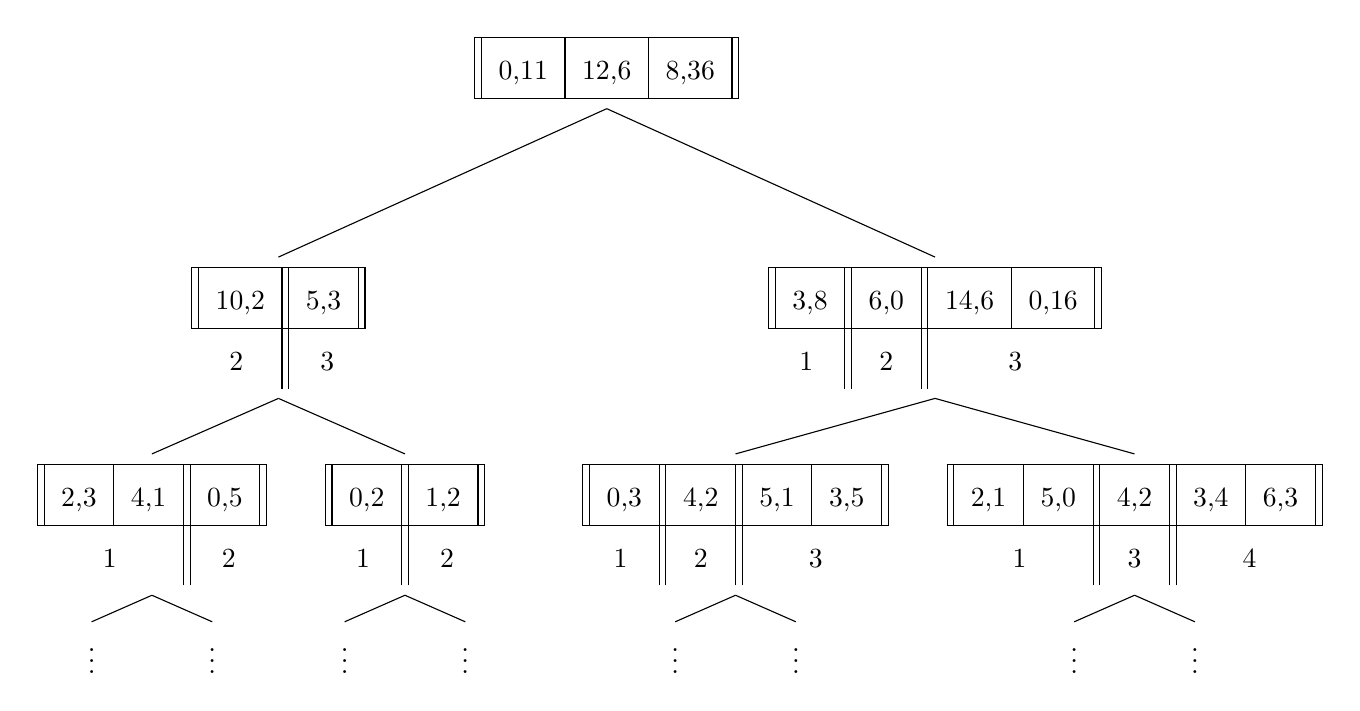
\begin{tikzpicture}[level 1/.style={level distance=3.3cm,sibling distance=1cm},
	level 2/.style={level distance=2.5cm,sibling distance=0.5cm},
	level 3/.style={level distance=1.8cm,sibling distance=1.2cm}]
  

\Tree [.{\begin{tabular}{||c|c|c||}  \hline 0,11 & 12,6 & 8,36 \\ \hline\end{tabular}}
 [.{\begin{tabular}{||c||c||}  \hline 10,2 & 5,3 \\  \hline \multicolumn{1}{c||}{2} & \multicolumn{1}{c}{3} \end{tabular}}
 [.{\begin{tabular}{||c|c||c||}\hline 2,3 & 4,1 & 0,5 \\\hline\multicolumn{2}{c||}{1} & \multicolumn{1}{c}{2}\end{tabular}} $\vdots$ $\vdots$ ]
  [.{\begin{tabular}{||c||c||}  \hline 0,2 & 1,2 \\  \hline \multicolumn{1}{c||}{1} & \multicolumn{1}{c}{2} \end{tabular}} $\vdots$ $\vdots$ ] ]
          [.{\begin{tabular}{||c||c||c|c||}  \hline 3,8 & 6,0 & 14,6 & 0,16 \\ \hline \multicolumn{1}{c||}{1} & \multicolumn{1}{c||}{2} & \multicolumn{2}{c}{3}\end{tabular}}
           [.{\begin{tabular}{||c||c||c|c||}  \hline 0,3 & 4,2 & 5,1 & 3,5 \\ \hline \multicolumn{1}{c||}{1} & \multicolumn{1}{c||}{2}& \multicolumn{2}{c}{3}\end{tabular}} $\vdots$ $\vdots$ ]
            [.{\begin{tabular}{||c|c||c||c|c||}  \hline 2,1 & 5,0 & 4,2 & 3,4 & 6,3 \\ \hline \multicolumn{2}{c||}{1} & \multicolumn{1}{c||}{3} & \multicolumn{2}{c}{4}\end{tabular}} $\vdots$ $\vdots$ ] ] ]

\end{tikzpicture}
\end{center}
\caption{\label{fig:block} Showing concurrent operation sets with blocks. Each block consists of a pair(left, right) indicating the number of operations from the left and the right child, respectively. Block (12,6) in the root contains blocks (10,2) from the left child and (6,0) from the right child. Blocks between two lines $||$ are propagated together to the parent. For example, Blocks (2,3) and (4,1) from the leftmost leaf and (0,2) from its sibling are propagated together into the block (10,2) in their parent. The number underneath a group of blocks in a node indicates which block in the node's parent those blocks were propagated to.}
\end{figure}


Each block $b$ in node $n$ is the aggregation of blocks in the  children of $n$ that are newly read by the\textsc{Propagate}() step that created block $b$. For example, the third block in the root (8,36) is created by merging block (5,3) from the left child and (14,6) and (0,16) from the right child. Block (5,3) also points to elements from blocks (0,5) and (1,2). 
%Recursively we can deduce each block contents until the leaf nodes store arrays of individual element operations.

\begin{definition}\{Existence of an operation in a block\}  Operation op exists in block b if it has propagated up to block b.
\end{definition}


\begin{definition}\{Subblock\}
  The blocks that are aggregated into block $b$ in a \textsc{Propagate}() step are called subblocks of $b$. Block $b_1$ is a subblock of $b_2$ if and only if $b_1$ is a block in node $v$ and in $b_2$ is a block in the parent of $v$ and $b_1$'s elements exits in $b_2$'s elements.
\end{definition}
%{\TODO: describe how blocks work with a good example how exactly it is done}

\paragraph{}
We choose to linearize operations in a block from the left child before those from the right child as a convention. Operations within a block of the root can be ordered in any way that is convenient. In effect, this means that if there are concurrent new blocks in a \textsc{Refresh}() step from several processes we linearize them in the order of their process ids. So for example  operations aggregated in block (10,2) are in the order (2,3),(4,1),(0,2). All blocks from the left child with come before the right child and the order of blocks of each child is preserved among themselves.
%\begin{lemma}
%\label{lem:block_size}
%There cannot be more than one operation from each process in a \textsc{Refresh}() invocation.
%\end{lemma}
%\begin{proof}
%  If so, then that parent process has invoked two simultaneous operations. $ \blacksquare $
%\end{proof}

\paragraph{}
In a \textsc{Propagate}() invocation path from a leaf to root, there will be \textsc{Refresh}() steps with merges from $2, 4, 8, ..., p$ processes. So in a complete propagation, at most $2p$ blocks are merged into one block. \texttt{(maybe useful for analysis)}
%\begin{lemma}
%A block in the root cannot contain more than one operation from a process.
%\end{lemma}
%\begin{proof}
%  Assume a process in a block invokes two operations; one has to be finished another. If so, it has been added to root before. $\blacksquare$
%\end{proof}

\subsection{Using pointers and prefix sum to make \textsc{GetIndex}($i$) faster}
%\begin{definition}
%  \textsc{BSearch}($i$): Search $i$th element in a prefix sum array with length $n$ in \textsc{O}($\log n$) steps.
%\end{definition}
\paragraph{}
\textsc{GetIndex}($i$) returns the $i$th operation stored in the block tree sequence. We do that by finding the block $b_i$ containing $i$th element in the root, and then recursively finding the subblock of $b_i$ which contains $i$th element. To make this recursive search faster, instead of iterating over all elements in sequence of blocks we store prefix sum of number of elements in the blocks sequence and pointers to make BSearch faster.

Furthermore, in each block, we store the prefix sum of left and right elements. Moreover, for each block, we store two pointers to the last left and right subblock of it (see fig \ref{fig::pointer} and \ref{fig:prefix}).

\begin{figure}
\begin{center}
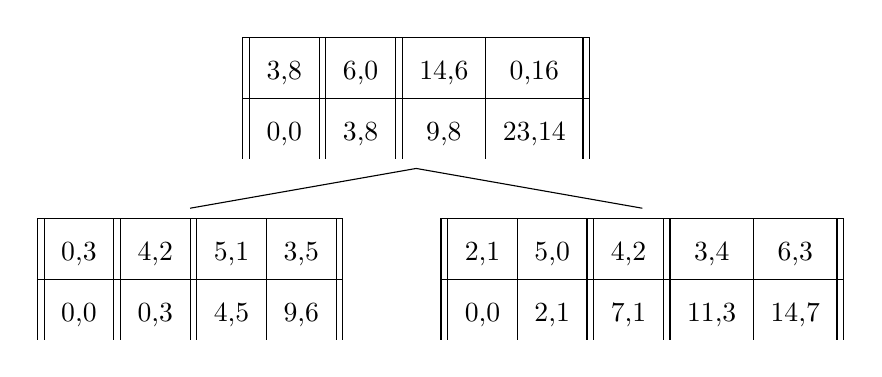
\begin{tikzpicture}[level 1/.style={level distance=2.3cm,sibling distance=1cm}]
  
\Tree [.{\begin{tabular}{||c||c||c|c||}  \hline 3,8 & 6,0 & 14,6 & 0,16 \\ \hline  0,0 & 3,8 & 9,8 & 23,14\end{tabular}}
           [.{\begin{tabular}{||c||c||c|c||}  \hline 0,3 & 4,2 & 5,1 & 3,5 \\ \hline 0,0 & 0,3 & 4,5 & 9,6 \end{tabular}} ]
            [.{\begin{tabular}{||c|c||c||c|c||}  \hline 2,1 & 5,0 & 4,2 & 3,4 & 6,3 \\ \hline 0,0 & 2,1 & 7,1 & 11,3 & 14,7 \end{tabular}} ] ]


\end{tikzpicture}
\end{center}
\caption{\label{fig:prefix} Using Prefix sums in blocks. When we want to find block b elements in its children, we can use binary search. The number below each block shows the count of elements in the previous blocks.}
\end{figure}

\begin{figure}[hbt]
\centering
  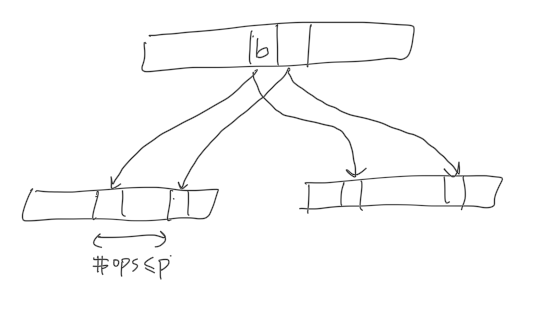
\includegraphics[width=5in]{pics/pointers}
  \caption{Block have pointers to the starting block of theirs for each child. \label{fig::pointer}}
\end{figure}

\paragraph{}
Starting from the root, \textsc{GetIndex}($i$) BSearches $i$ in the prefix sum array to find block containing $i$th operation, then continues recursively calling \textsc{GetElement}($b,i$) to find $i$th element of block $b$. From lemma $\ref{lem:block_size}$ we know a block size is at most $p$. So BSearch takes at most \textsc(O)$(\log p)$, since  with knowing pointers of a block and its previous block we can determine the base \texttt{(domain ?)} to search and its size is \textsc{O}$(p)$.

\subsection{Block Tree Algorithm}
\paragraph{}
Our Block Tree is a linearizable implementation of a data structure that stores a sequence of elements. It has two methods (see Algorithm~\ref{alg2}), \textsc{Append}($e$) which appends element $e$ to the sequence, and \textsc{Get}($i$) which returns the $i$th element in the sequence.

\paragraph{Design of a block tree}

Each process is assigned to a leaf in a shared tournament tree. Thus, for example, the leaf node for process $p_i$ contains an array of elements by $p_i$ in the order they were invoked.
Each internal node of the tree contains an array of blocks of elements.
Block $b$ in node $n$ is created in a \textsc{Propagate}() step and is merged block of new blocks at the time of \textsc{Propagate}() reading $n$'s children blocks. Each block consists of pointers left and right, to the last block merged into itself from left and right child in that order. Moreover, two numbers, left and right, indicate the count of elements in the blocks from the left and right child consecutively. Furthermore, prefix left, and right can be computed from the prefix sum of left and right values.
Elements of block $b$ can be determined recursively (\textsc{GetElements($b$)}).
The $i$th element in the sequence can be determined in \textsc{O}($\log^2 p$) steps by recursively finding $i$th element in block $b$ (\textsc{GetElement($i$)})
After element $e$ is propagated (appended to a block int the root), its index can be computed with \textsc{GetIndex}($op$).


In order to compute elements of a block faster we store prefix-sum blocks(block i has tuple(right-sum=$\#$right ops in previous block, left-sum=$\#$left ops in previous blocks)[See Figure \ref{fig:prefix}]. Here is the algorithm to get elements of a block.

\paragraph{Specification}
A block tree is a shared data structure that stores a sequence of elements.  It has two methods \texttt{Append(e)} and \texttt{Get(i)}. \texttt{Append(e)} adds \texttt{e} to the end of the sequence and returns the index of \texttt{e} in the sequence. \texttt{Get(i)} returns \texttt{i}th element stored in the sequence. 

\paragraph{SubBlock} Block \texttt{s} is a subblock of \texttt{b} if \texttt{s} is between blocks \texttt{start..end} in \texttt{n} from Lines 41,42 of \texttt{CreateBlock()}.

\paragraph{Membership}
Element \texttt{e} is a member of block \texttt{b} in:
\begin{itemize}
  \item internal node \texttt{n}, if \texttt{e} is a memeber of \texttt{s} that \texttt{s} is a subblock of \texttt{b}.
  \item leaf node \texttt{n}, if \texttt{e} belongs to \texttt{n.dir.blocks[b\textsuperscript{$\prime$}.end\textsubscript{dir}+1..b.end\textsubscript{dir}]} for \texttt{dir} $\in$ \texttt{\{left, right\}} which b\textsuperscript{$\prime$} is the previous block of \texttt{b} in \texttt{n}.
\end{itemize}

\paragraph{Order of elements inside node}
Element \texttt{d} is before element \texttt{e} in node \texttt{n}, if:
\begin{itemize}
  \item The block containing d is before the block containing e.
  \item e and d are in the same block and d is in the left child and e is in the right child.
  \item d is before e in the same child's order.
\end{itemize}


\begin{figure}[hbt]
  \center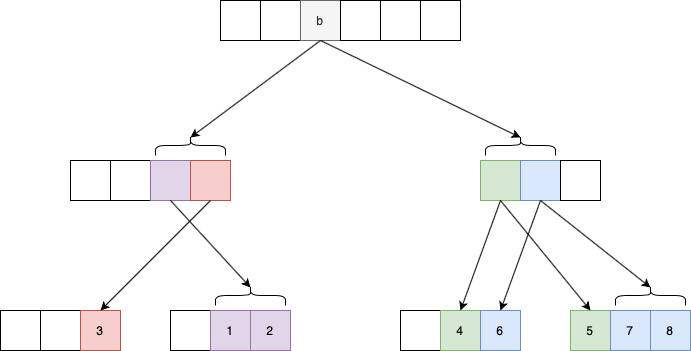
\includegraphics[width=5.5in]{pics/tree}
  \caption{Order of elements in b: elements in leaves are ordered with numerical order in the drawing.}
\end{figure}


\paragraph{\texttt{CreateBlock()}} \texttt{CreateBlock(n)} returns a block containing new operations of \texttt{n}'s children. \texttt{b\textsuperscript{$\prime$}.end\textsubscript{left}} stores the index of the rightmost subblock of left child of \texttt{b}'s previous block. Other attributes are assigned values followed by definition.
\begin{figure}[hbt]
  \center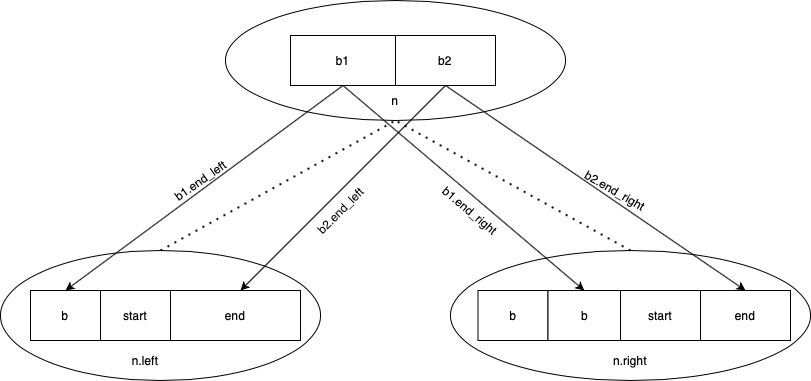
\includegraphics[width=5.5in]{pics/createblock}
  \caption{\label{fig::createBlock}Snapshot of a CreateBlock()}
\end{figure}

%\textsf{Is it necessary to say \texttt{CreateBlock()} is doing what it's supposed to do by definition? Or \texttt{Append()} for example?}


\paragraph{Double Refresh}
Elements in \texttt{n}'s children's blocks before line \texttt{13} are guaranteed to be in \texttt{n}'s blocks after Line~\texttt{15}.
\begin{proof}
\texttt{CreateBlock()} reads blocks in the children that does not exist in the parent and aggregates them into one block. If a \texttt{Refresh} procedure returns true it means it has appended the block created by \texttt{CreateBlock()} into the parent node's sequence. So suppose two \texttt{Refresh}es fail. Since the first \texttt{Refresh} was not successful, it means another CAS operation by a \texttt{Refresh}, concurrent to the first\texttt{Refresh}, was successful before the second \texttt{Refresh}. So it means the second failed \texttt{Refresh} is concurrent with a successful \texttt{Refresh} that assuredly has read block before the mentioned line \texttt{13}. After all it means if any of the \texttt{Refresh} attempts were successful the claim is true, and also if both fail the mentioned claim still holds.
\end{proof}
\begin{figure}[hbt]
  \center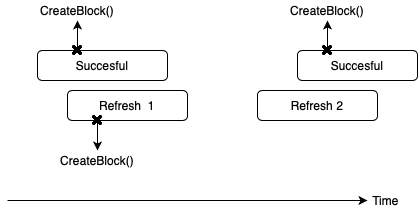
\includegraphics[width=4in]{pics/doublerefresh.png}
  \caption{The second failed Refresh is assuredly concurrent to a Successful \texttt{Refresh()} with \texttt{CreateBlock} line after first failed \texttt{Refresh}'s \texttt{CreateBlock()}.}
\end{figure}


\paragraph{Disjunction} Blocks in node \texttt{n}'s contain disjoint sets of elements.
\begin{proof}
Without loss of generality, assume blocks \texttt{b1, b2} contain common element \texttt{e} from the left child, and \texttt{b2} is after \texttt{b1} in \texttt{n}'s sequence of blocks. So block start of b2's \texttt{CreateBlock()} is after block end of \texttt{b1}'s end. Since \texttt{b2}'s start is the end of the block before itself, it cannot be before \texttt{b1}'s end.
\end{proof}

\paragraph{Total Order}
Sequence represented by the Block Tree is the sequence of the blocks stored in the root.

\paragraph{Linearization Points}
\texttt{Get(i)} is linearized when it terminates. \texttt{Append(e)} is linearized right after when a block containing \texttt{e} is appended to the root, if there are multiple elements appended together, they are linearized by the defined order in the root.

\paragraph{Subblocks Upperbound} Block b has at most $p$ subblocks.
\begin{proof}
If there are more than $p$ subblocks, then there is more than one block from process pl. \texttt{Append(e)} finishes after propagating and appending \texttt{e} to the root(line 9). So these blocks cannot be appended to root already, so pl has invoked two concurrent \texttt{Append()}s(line 1) without terminating the first one.
\end{proof}

\paragraph{Computing \texttt{Get(n, b, i)}}
To find the \texttt{i}th element in block \texttt{b} of node \texttt{n}, we search among subblocks of \texttt{b} that is bounded by $p$. Subblocks of a block are within the start and end block of the \texttt{CreateBlock()} procedure of it.

\paragraph{How \texttt{Refresh(n)} works.}
\begin{enumerate}
  \item Read n's counter and head
  \item Create block b
  \item CAS b into n
  \item If previous succeed:
  \begin{enumerate}
  \item Update sup of b's ending subblocks
  \item Increment children's counters
  \end{enumerate}
\end{enumerate}


%\paragraph{Time-Space Relation} There are at most $p^2$ blocks with same \texttt{time} attribute.
%\begin{proof}
%If a process dies at line 28, the children counter won't increase, and each process aggregates most block, and since there are at most p concurrent processes, then there will be at most $p^2$ blocks with same \texttt{time} attribute.
%\end{proof}
%
%\paragraph{Time-Propagate() Relation} In a \texttt{CreateBlock()} procedure, the blocks that are seen have at most 2 different \texttt{time} attribute values.
%
%\paragraph{Time-Super Relation} sup[i+1]-sup[i] is $\leq p$
%
%\paragraph{\texttt{b}'s Superblock position} SuperBlock of \texttt{b} is within range $\pm p$ of the \texttt{\texttt{sup[b.time]}}.
%\begin{proof}
%
%\end{proof}
\begin{figure}[hbt]
  \center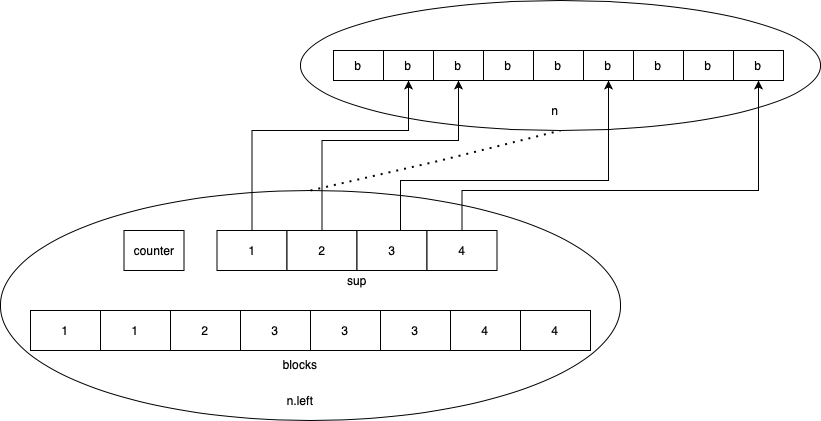
\includegraphics[width=6in]{pics/super}
  \caption{\texttt{Sup} and \texttt{timer} in a node, numbers on blocks are their \texttt{time} values.}
\end{figure}

\paragraph{Computing superblock}
\begin{enumerate}
  \item Value read for \texttt{super[b.time]} in line 71 is not null.\begin{proof}
    \texttt{Index()} is invoked after finishing \texttt{Propagate()} in line 10. For each value \texttt{c\textsubscript{dir}} read in lines 23, \texttt{super} is set before incrementing in lines 26,27.
  \end{proof} 
  \item \texttt{super[]} preserves order from child to parent; if in a child block \texttt{b} is before \texttt{c} then \texttt{b.time} $\leq$ \texttt{c.time} and \texttt{super[b.time]} $\leq$ \texttt{super[c.time]}\begin{proof}
   Follows from the order of lines 37, 26, 27.
 \end{proof}
%  \item In a propagate step at most 2 different time values are read \\ If there are more than 2 numbers then the smallest number should have been propagated far before.
%  \item There are at most $p^2$ blocks with same time value in a node. \\ At most p processes could die before line 27 and each contains at most p elements.
  \item \texttt{super[i+1]-super[i]}$\leq p$
\begin{proof}
 In a Refresh with successful CAS in line 24, \texttt{super} and \texttt{counter} are set for each child in lines 26,27. Assume the current value of the counter in node \texttt{n} is \texttt{i+1} and still \texttt{super[i+1]} is not set. If an instance of successful \texttt{Refresh(n)} finishes \texttt{super[i+1]} is set a new value and a block is added after \texttt{n.parent[sup[i]]}. There could be at most $p$ successful unfinished concurrent instances of \texttt{Refresh()} that have not reached line 27. So the distance between \texttt{super[i+1]} and \texttt{super[i]} is less than $p$.
 \end{proof}
  \item Superblock of \texttt{b} is within range $\pm 2p$ of the \texttt{super[b.time]}.
\begin{proof}
\texttt{super[i]} is the index of the superblock of a block containing block b. It is trivial to see that \texttt{n.super} and \texttt{n.b.counter} are increasing.  \texttt{super(b)} is the real superblock of b. \texttt{super(t]} is the index of the superblock of the last block with time \texttt{t}. If \texttt{b.time} is \texttt{t} we have:
$$super[t]-p\leq super[t-1]\leq super(t-1] \leq super(b) \leq super(t+1)\leq super(t+1]\leq super[t]+p$$
  \end{proof} 
\end{enumerate}

%The block tree contains a tournament tree in which leaves are assigned to processes, and each process appends elements to its leaf and tries to propagate it up to the root. The final sequence is stored at the root. \texttt{Append} after appending to leaf calls \texttt{Propagate} which iterates over the path to root. In each \texttt{Propagate(n)} invocation on node n it tries ti \texttt{Refresh} the sequence stored at node n with the new elements in n's children. After adding the element to the root \texttt{Index(op)} finds the order of the element in the root.

 

%\textsf{I finally thought maybe a sequence of elements is better for telling specification.}

\begin{algorithm}
\caption{Block Tree \label{alg2}}
\begin{algorithmic}[1]
\begin{multicols}{2}

\Statex \textbf{Structure}

\Statex $\blacktriangleright$ \texttt{\textsl{element} e}
\begin{itemize}
%\item \texttt{\textsl{string} name}
\item \texttt{\textsl{int} pid}
\item \texttt{\textsl{int} loc\textsf{: location in \texttt{l\textsubscript{pid}}.ops}}
\end{itemize}


\Statex $\blacktriangleright$ \texttt{\textsl{node} n}
\begin{itemize}
\item \texttt{\textsl{*node} left, right, parent}
\item \texttt{\textsl{block[]} blocks}\textsf{: blocks stored in \texttt{n}}
\item \texttt{\textsl{int} head= 1}\textsf{: index of first empty cell of \texttt{blocks}}
\item \texttt{\textsl{int} counter= 0}\textsf{}
\item \texttt{\textsl{int[]} super}\textsf{: \texttt{super[i]} stores the index of a superblock in parent that contains some block of this node whose \texttt{time} is \texttt{i}}
\end{itemize}

\Statex $\blacktriangleright$ \texttt{\textsl{leaf node} l\textsubscript{i} extends \textsl{node}}
\begin{itemize}
\item \texttt{\textsl{operation[]} ops}\textsf{: elements that are invoked to \texttt{Append()} to the blok tree by process i}
\end{itemize}


\Statex $\blacktriangleright$ \texttt{\textsl{block} b}
\begin{itemize}
  \item \texttt{\textsl{int} num\textsubscript{left}, sum\textsubscript{left}}
  
  \textsf{~~\#operations from the left subblocks of b, prefix sum of num\textsubscript{left}}

  \item \texttt{\textsl{int} num\textsubscript{right}, sum\textsubscript{right}}
  
  \textsf{~\#operations from the right subblocks of b, prefix sum of num\textsubscript{right}}
  
  \item \texttt{\textsl{int} sum}
  
  \textsf{\# operation in b}
  
  \item \texttt{\textsl{int} end\textsubscript{left}, end\textsubscript{right}}
  
  \textsf{~~index of \texttt{b}'s last subblock}
  \item \texttt{\textsl{int} time}

\end{itemize}


%\Statex \textbf{Examples}
%\Statex \hspace{0pt} \texttt{ l\textsubscript{i}[j]}\textsf{: jth operation of ith process}
%\Statex \hspace{0pt} \texttt{ n.left}\textsf{: left child of node n}
%\Statex \hspace{0pt} \texttt{ n.blocks[n.head]}\textsf{: leftmost empty block of node n}
%\Statex \hspace{0pt} \texttt{ n.blocks[i].num\textsubscript{left}}\textsf{: \#left operations of ith block of n}
%\Statex \hspace{4pt} \texttt{b.end\textsubscript{right}}\textsf{: index of ending right subblock of b}

\Statex

\Function{int}{Append}{\textsl{operation} op, \textsl{int} pid} 
\State \texttt{op.loc= l\textsubscript{pid}.head}
\State \texttt{block b= \Call{new}{\textsl{block}}}
\State \texttt{b.time= op.loc}
\State \texttt{b.sum= 1}
\State \texttt{l\textsubscript{pid}.ops[op.loc]= op}
\State \texttt{l\textsubscript{pid}.blocks[op.loc]= b}
\State \texttt{op.head+= 1}
\State \Call{Propagate}{l\textsubscript{pid}.parent}
\State \Return \Call{Index}{l\textsubscript{pid}, op.loc, b} 
\EndFunction{Append}

\columnbreak

\Function{void}{Propagate}{\textsl{node} n}
\If{\texttt{not} \Call{Refresh}{n}}
\State \Call{Refresh}{n}
\EndIf
\If{\texttt{n {\keywordfont is} root}} \Return
\EndIf
\State \Call{Propagate}{n.parent}
\EndFunction{Propagate}

\Statex

\Function{boolean}{Refresh}{\textsl{node} n}
\State \texttt{i= n.head}
\State \texttt{c= n.counter}
\State \texttt{new, c\textsubscript{left}, c\textsubscript{right}= \Call{CreateBlock}{n, i+1, c}}
\If{\Call{CAS}{n.blocks[i+1], null, new}}
\ForEach{\texttt{dir} {\keywordfont{in}} \texttt{\{left, right\}}}
\State \texttt{\Call{CAS}{n.dir.super[c\textsubscript{dir}], null, i+1}}
\State \texttt{\Call{CAS}{n.dir.counter, c\textsubscript{dir}, c\textsubscript{dir}+1}}
\EndFor
\State \Return{\texttt{true}}
\Else 
\State \Return{ \texttt{false}}
\EndIf
\State \texttt{\Call{CAS}{n.head, i, i+1}}
\EndFunction{Index}

\Statex

\Function{block, int, int}{CreateBlock}{\textsl{node} n, \textsl{int} i, int c} 
\Statex\Comment{Creates a block to insert into \texttt{n.blocks[i]}}
\State \texttt{block b= \Call{new}{\textsl{block}}}
\State \texttt{b.time= c}
\ForEach{\texttt{dir} {\keywordfont{in}} \texttt{\{left, right\}}}
\State \texttt{j= n.dir.head}
\State \texttt{start= n.blocks[i-1].end\textsubscript{dir}}
\State \texttt{end= n.dir.blocks[j]}
\State \texttt{c\textsubscript{dir}= n.dir.blocks[j].time}
\State \texttt{b.end\textsubscript{dir}= j}
\State \texttt{b.num\textsubscript{dir}= end.sum - start.sum}
\State \texttt{b.sum\textsubscript{\#dir}= n.blocks[i-1].sum\textsubscript{\#dir} + b.num\textsubscript{dir}}
\EndFor
\State \texttt{b.sum= b.sum\textsubscript{left} + b.sum\textsubscript{right}}
\State \Return \texttt{b, c\textsubscript{left}, c\textsubscript{rightt}}
\EndFunction{CreateBlock}


\end{multicols}
\end{algorithmic}
\end{algorithm}

\begin{algorithm}
\caption{Block Tree Continued}
\begin{algorithmic}[1]
\setcounter{ALG@line}{46}

\Function{element}{Get}{\textsl{int} i} 
\State \texttt{res= \Call{BSearch}{root, sum, i, 0, root.head}}
\State \Return{\Call{Get}{root, res, i-root.blocks[res-1].sum}}
\EndFunction{Get}

\Statex


\Statex $\leadsto$ \textsf{Precondition: \texttt{n.blocks[start..end]} contains a block with field \texttt{f} $\geq$ \texttt{i}}
\Function{int}{BSearch}{\textsl{node} n, \textsl{field} f, \textsl{int} i, \textsl{int} start, \textsl{int} end}

\Statex \Comment{\textmd{Searches~the value \texttt{i} of the given prefix sum \texttt{type} on the node \texttt{n} in the domain from \texttt{start} to \texttt{end} blocks. \texttt{f} is one of \texttt{sum, sum\textsubscript{left}, sum\textsubscript{right}}. Does binary search on \textsl{field} \texttt{f} of the blocks stored in \texttt{n.blocks} and returns the index of the leftmost block in \texttt{n.blocks[start..end]} whose \textsl{field} \texttt{f} is $\geq$ \texttt{i}}.}
\State \Return \texttt{result block's index}
\EndFunction{BSearch}

\Statex

\Function{element}{Get}{\textsl{node} n, \textsl{int} b, \textsl{int} i} 
\Comment{\textmd{Returns the \texttt{i}th operation in \texttt{b}th block of node \texttt{n}}}
\If{\texttt{n {\keywordfont is} leaf}} \Return \texttt{n.ops[i]}
\Else
\If{\texttt{i $\leq$ n.blocks[b].num\textsubscript{left}}} \Comment{\texttt{i} exists in left child of \texttt{n}}
\State \texttt{subBlock= \Call{BSearch}{n.left.sum, i, n.blocks[b-1].end\textsubscript{left}+1, n.blocks[b].end\textsubscript{left}}}
\State \Return\Call{Get}{n.left, subBlock, i-n.left.blocks[subBlock-1].sum} 
\Else
\State \texttt{i= i-n.blocks[b].num\textsubscript{left}}
\State\texttt{subBlock=\Call{BSearch}{n.right.sum, i, n.blocks[b-1].end\textsubscript{right}, n.blocks[b].end\textsubscript{right}}}
\State \Return\Call{Get}{n.right, subBlock, i-n.right.blocks[subBlock-1].sum} 
\EndIf
\EndIf
\EndFunction{Get}

\Statex
\Statex $\leadsto$ \textsf{Precondition:~\texttt{i}th operation in node \texttt{n} is in block \texttt{b} of node \texttt{n}.}
\Function{index}{Index}{\textsl{node} n, \textsl{int} i, \textsl{int} b} \Comment{Returns rank in the  
root of the \texttt{i}th operation in node \texttt{n}.}
\If{\texttt{n {\keywordfont is} root}} \Return \texttt{i}
\Else
\State \texttt{dir= (n.parent.left==n)? left: right}
\State \texttt{superBlock= \Call{BSearch}{n.parent, n.sum\textsubscript{dir}, i, sup[n.blocks[b].time]-p, sup[n.blocks[b].time]+p}}
\If{\texttt{dir {\keywordfont is} left}}
\State \texttt{i+= n.parent.blocks[superBlock-1].sum\textsubscript{right}}
\Else \State \texttt{i+= n.parent.blocks[superBlock].sum\textsubscript{left} + n.parent.blocks[superBlock].sum\textsubscript{left} + n.blocks[nBlock-1].sum}
\EndIf
\State \Return\Call{Index}{n.parent, i, superBlock}
\EndIf
\EndFunction{Index}

\Statex

%\Function{list}{GetElements}{block b} 
%\ForEach{block {\keywordfont in} \Call{GetSubBlocks}{b}}
%\State result.append(\Call{GetElements}{})
%\EndFor
%\State \Return result
%\EndFunction{GetElements}
%
%\Statex
%
%\Function{list}{GetSubBlocks}{b}
%\State n:=b.node
%\State b[-1]=b's previous block
%\ForEach{direction \{left, right\}}
%\State init=\Call{BSearch}{n.direction, b[-1].direction}
%\State end=\Call{BSearch}{n.direction, b.direction}
%\State result.append([init:end])
%\EndFor
%\State \Return result
%\EndFunction{GetSubBlocks}

\end{algorithmic}
\end{algorithm}

\section{Implementing Queue using Block Tree}
\subsection{Idea in a nutshell}
With the ideas introduced in block tree we are going to create a shared wait-free queue with \textsc{O}$(\log ^2p+\log n)$ steps. A queue stores a sequence of elements and supports two operations, enqueue and dequeue. \texttt{Enqueue(e)} appends element \texttt{e} to the sequence stored.\texttt{Dequeue()} removes and returns the first element among in the sequence. If the queue is empty it returns \texttt{null}. Knowing index $i$ is the tail of the queue, we can return the dequeue response using \texttt{Get(i)}.  So in the rest we modify block tree to compute \texttt{i} for each \texttt{Dequeue()} to achieve a FIFO queue.
%
%\subsection{What should a \texttt{Dequeue()} return, regarding history of operations?}
\paragraph{}
Next, we describe how to use block tree to implement queues. The block tree, maintains the history of all operations, not only the current state of the queue. Now consider the following history of operations. What should each \texttt{Dequeue()} return?

\begin{table}[hbt]
\centering
  \begin{tabular}{c|c|c|c|c|c|c|c|c|c}
    \hline \texttt{ENQ(5)}& \texttt{ENQ(2)}& \texttt{DEQ()}& \texttt{ENQ(3)}&\texttt{DEQ()}& \texttt{DEQ()}& \texttt{DEQ()}& \texttt{ENQ(4)}& \texttt{ENQ(6)}& \texttt{DEQ()}\\ \hline
  \end{tabular}
  \caption{An example histoy of operations on the queue}
\end{table}

\begin{definition}
A non-null dequeue is one that returns a non-null value.
\end{definition}

\paragraph{}
In the example above, \texttt{Dequeue()} operations return \texttt{5, 2, 3, null, 4} in order. Before \texttt{ENQ(4)} the queue gets empty so the last \texttt{DEQ()} returns null. If the queue is non-empty and $r$ \texttt{Dequeue()} operations have returned a non-null response, then $i$th \texttt{Dequeue()} returns the input of the $r+1$th \texttt{Enqueue()}. So, in order to answer a Dequeue, it's sufficent to know the size of the queue and the number of previous non-null dequeues.

%\texttt{DEQ[i] = (size>0) ? ENQ[r+1] : null;}


%\subsection{What should a \texttt{Dequeue()} return, regarding history of blocks of operations?}

\paragraph{}
In the Block Tree, we did not store the sequence of operations explicitly but instead stored blocks of concurrent operations to optimize \texttt{Propagate()} steps and increase parallelism. So now the problem is to find the result of each Dequeue. From lemma \ref{lem:block_size} we know we can linearize operations in a block in any order; here, we choose to decide to put Enqueue operations in a block before Dequeue operations. In the next example, operations in a cell are concurrent. \texttt{DEQ()} operations return \texttt{null, 5, 2, 1, 3, 4, null} respectively. We will next describe how these values can be computed efficiently.

\begin{table}[hbt]
\centering
  \begin{tabular}{c|c|c|c}
    \hline \texttt{DEQ()} & \texttt{ENQ(5)}, \texttt{ENQ(2)}, \texttt{ENQ(1)}, \texttt{DEQ()}& \texttt{ENQ(3)}, \texttt{DEQ()}&  \texttt{ENQ(4)}, \texttt{DEQ()}, \texttt{DEQ()}, \texttt{DEQ()}, \texttt{DEQ()}\\ \hline
  \end{tabular}
  \caption{An example history of operation blocks on the queue}
\end{table}

\paragraph{}
Now, we claimed that by knowing the current size of the queue and the number of non-null dequeue operations before the current dequeue, we could compute the index of the resulting \texttt{Enqueue()}. We apply this approach to blocks; if we store the size of the queue after each block of operations happens and the number of non-null dequeues dequeues till a block, we can compute each dequeue's index of result in \textsc{O}$(1)$ steps.

\begin{table}[hbt]
\centering
  \begin{tabular}{c|c|c|c|c}
    \hline &\texttt{DEQ()} & \texttt{ENQ(5)}, \texttt{ENQ(2)}, \texttt{ENQ(1)}, \texttt{DEQ()}& \texttt{ENQ(3)}, \texttt{DEQ()}&  \texttt{ENQ(4)}, \texttt{DEQ()}, \texttt{DEQ()}, \texttt{DEQ()}, \texttt{DEQ()}\\ \hline
    \#enqueues & 0 & 3 & 1 & 1 \\ \hline
        \#dequeues & 1 & 1 & 1 & 4 \\ \hline
            \#non-null dequeues & 0 & 1 & 2 & 5 \\ \hline
                size & 0 & 2 & 2 & 0 \\ \hline
  \end{tabular}
  \caption{Augmented history of operation blocks on the queue}
\end{table}

%\begin{definition}
%  \texttt{index(op)}: index of the given Dequene among same type operation in conataing block.
%  
%  \texttt{INDEX(op)}: index of the given Dequene among same type operation in all operations.
%  
%\end{definition}

Size and the number of non-null dequeues for $b$th block could be computed this way:\\
\texttt{size[b]= max(size[b-1] +enqueues[b] -dequeues[b], 0)}\\
\texttt{non-null dequeues[b]= non-null dequeues[b-1] +dequeues[b] -size[b-1] -enqueues[b]}

Given \texttt{DEQ} is in block \texttt{b}, \texttt{response(DEQ)} would be:\\
\texttt{(size[b-1]- index of DEQ in the block's dequeus >=0) ? ENQ[non-null dequeus[b-1]+ index of DEQ in the block's dequeus] : null;}

\section{Main Algorithm}

\paragraph{Specification}
A Queue is a shared data structure that stores a sequence of elements. It has two methods \texttt{Enqueue(e)} and \texttt{Dequeue()}. \texttt{Enqueue(e)} adds \texttt{e} to the end of the sequence. \texttt{Dequeue()} returns the first element stored in the sequence and removes it from the sequence.


%Now that we know how to augment Block Tree root history to compute the response, we will present the complete algorithm. \texttt{Enqueue()} and \texttt{Dequeue()} are the main functions. \texttt{Enqueue(e)} adds \texttt{e} to the queue and \texttt{Dequeue()} returns the first element in the queue and removes it from the queue. Block Tree functionalities are very similar. \texttt{Append(e)} does what \texttt{Enqueue()} does and if we know the current index of the head of the queue we can call \texttt{Get()} to find its value.

\begin{figure}[hbt]
\centering
  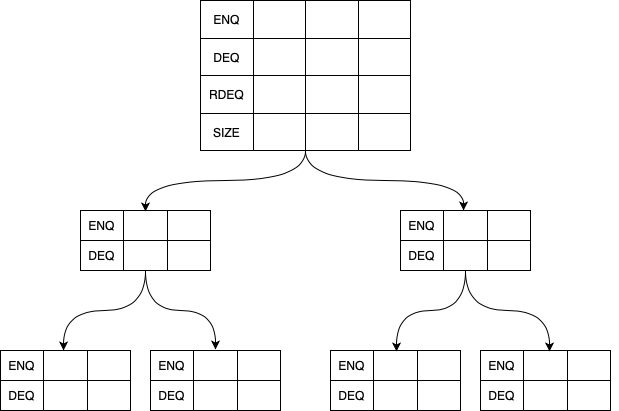
\includegraphics[width=5in]{pics/queue}
  \caption{Fields stored in the Queue nodes. \label{fig::queue}}
\end{figure}


\begin{algorithm}
\caption{Queue \label{algQ}}
\begin{algorithmic}[1]
\begin{multicols}{2}

%\Statex \textbf{Structure}

\Statex $\blacktriangleright$ \texttt{\textsl{Operation}}
\begin{itemize}
%\item \texttt{\textsl{string} name}
%\item \texttt{\textsl{string} type$\in$\{DEQ,ENQ\}}
\item \texttt{\textsl{Object} element}\textsf{: argument of an enqueue, if null this is a dequeue}
%\item \texttt{\textsl{int} pid}
\item \texttt{\textsl{int} loc\textsf{: location in the leaf's \texttt{ops}}}
\end{itemize}


\Statex $\blacktriangleright$ \texttt{\textsl{Node}}
\begin{itemize}
\item \texttt{\textsl{*Node} left, right, parent}
\item \texttt{\textsl{Block[]} blocks}\textsf{: index 0 contains an empty block with all fields equal to 0}
\item \texttt{\textsl{int} head= 1}\textsf{: index of the first empty cell of \texttt{blocks}}
\item \texttt{\textsl{int} counter= 0}\textsf{}
\item \texttt{\textsl{int[]} super}\textsf{: \texttt{super[i]} stores the index of a superblock in parent that contains some block of this node whose \texttt{time} is field \texttt{i}}
\end{itemize}

\Statex $\blacktriangleright$ \texttt{\textsl{Leaf} extends \textsl{Node}}
\Statex \Comment{\textsf{\texttt{l\textsubscript{i}} is the Leaf for process \texttt{i} and \texttt{i} is in range \texttt{0} to \texttt{p-1}}}
\begin{itemize}
\item \texttt{\textsl{Operation[]} ops}\textsf{: invoked operations}
\end{itemize}

\Statex $\blacktriangleright$ \texttt{\textsl{Root} extends \textsl{Node}}
\begin{itemize}
\item \texttt{override \textsl{Root Block[]} blocks}
\end{itemize}


\Statex $\blacktriangleright$ \texttt{\textsl{Block}}

\begin{itemize}
  \item \texttt{\textsl{int} num\textsubscript{enq-left}, sum\textsubscript{enq-left}}
  
  \textsf{~~\#enqueues from subblocks in left child, prefix sum of \texttt{num\textsubscript{enq-left}}}

  \item \texttt{\textsl{int} num\textsubscript{deq-left}, sum\textsubscript{deq-left}}
  
  \textsf{~~\#dequeues from subblocks in left child, prefix sum of \texttt{num\textsubscript{deq-left}}}


  \item \texttt{\textsl{int} num\textsubscript{enq-right}, \texttt{sum\textsubscript{enq-right}}}
  
  \textsf{~\#enqueues from subblocks in right child, prefix sum of \texttt{num\textsubscript{enq-right}}}
  
  \item \texttt{\textsl{int} num\textsubscript{deq-right}, \texttt{sum\textsubscript{deq-right}}}
  
  \textsf{~\#dequeues from subblocks in right child, prefix sum of \texttt{num\textsubscript{deq-right}}}

  
  \item \texttt{\textsl{int} num\textsubscript{enq}, num\textsubscript{deq}}
  
  \textsf{\# enqueue, dequeue operations in the block}

  \item \texttt{\textsl{int} sum\textsubscript{enq}, sum\textsubscript{deq}}
  
  \textsf{sum of \# enqueue, dequeue operations in blocks up to this one}
  
  \item \texttt{\textsl{int} num, sum}
  
  \textsf{total \# operations in block, prefix sum of \texttt{num}}
  
  \item \texttt{\textsl{int} end\textsubscript{left}, end\textsubscript{right}}
  
  \textsf{~~index of this block's last subblock in the left and right child}
  \item \texttt{\textsl{int} group}

\end{itemize}

\Statex $\blacktriangleright$ \texttt{\textsl{Root Block} extends \textsl{Block}}
\begin{itemize}
  \item \texttt{\textsl{int} size}
  
  \textsf{size of queue after this block's operations finish}

  \item \texttt{\textsl{int} sum\textsubscript{non-null deq}}
  
  \textsf{count of non-null dequeus up to this block}


\end{itemize}


%\Statex \textbf{Examples}
%\Statex \hspace{0pt} \texttt{ l\textsubscript{i}[j]}\textsf{: jth operation of ith process}
%\Statex \hspace{0pt} \texttt{ n.left}\textsf{: left child of node n}
%\Statex \hspace{0pt} \texttt{ n.blocks[n.head]}\textsf{: leftmost empty block of node n}
%\Statex \hspace{0pt} \texttt{ n.blocks[i].num\textsubscript{left}}\textsf{: \#left operations of ith block of n}
%\Statex \hspace{4pt} \texttt{b.end\textsubscript{right}}\textsf{: index of ending right subblock of b}

\Statex

\Function{void}{Enqueue}{\textsl{Object} e}
\State \texttt{op= NEW(\textsl{operation})}
%\State \texttt{op.type= ENQ}
\State \texttt{op.element= e}
%\State \texttt{op.pid= this.pid}
\State \Call{Append}{op}
\EndFunction{Enqueue}

\Statex

\Function{Object}{Dequeue()}{}
\State \texttt{op= NEW(\textsl{operation})}
%\State \texttt{op.type= DEQ}
%\State \texttt{op.pid= this.pid}
\State  \Call{Append}{op} \Comment{$i$th DEQ in $b$th block}
\State \texttt{<i, b>=} \Call{Index}{l\textsubscript{pid}, op.loc, 1}
\State \texttt{res=} \Call{ComputeHead}{i, b} \Comment{Index of the enqueue whose argument should be returned}
\If{\texttt{res }\textbf{is }\texttt{null}}
\State \Return \texttt{null}
\Else
\State \Return \Call{Get}{res}
\EndIf
\EndFunction{Dequeue}

\Statex

\Function{int}{ComputeHead}{int i, int b}\Comment{Computes head of the queue when \texttt{i}th dequeue in \texttt{b}th block occurs. The dequeue should return the argument of the head enqueue.}
\If{\texttt{root.blocks[b-1].size + root.blocks[b].num\textsubscript{enq} - i $<$ 0}}
\State \Return \texttt{-1}
\Else{ \Return \texttt{root.blocks[b-1].sum\textsubscript{non-null deq} + i}}
\EndIf
\EndFunction{ComputeHead}

\Statex

\Function{void}{Append}{\textsl{operation} op} 
\State \texttt{pid= id of process performing \textsc{Append}}
\State \texttt{op.loc= l\textsubscript{pid}.head}
\State \texttt{op.head+= 1}
\State \texttt{block b= \Call{new}{\textsl{block}}}
\State \texttt{b.group= op.loc}
\If{\texttt{op.element==null}} 
\texttt{b.sum\textsubscript{deq}=1} \Else \texttt{~b.sum\textsubscript{enq}=1} \EndIf
%\State \texttt{b.sum\textsubscript{op.type}= 1}
\State \texttt{l\textsubscript{pid}.ops[op.loc]= op} \label{addOP}
\State \texttt{l\textsubscript{pid}.blocks[op.loc]= b}
\State \Call{Propagate}{l\textsubscript{pid}.parent} 
\EndFunction{Append}

\end{multicols}
\end{algorithmic}
\end{algorithm}

\begin{algorithm}
\caption{Queue Continued}
\begin{algorithmic}[1]
\setcounter{ALG@line}{33}
\begin{multicols}{2}

\Function{void}{Propagate}{\textsl{node} n}
\If{\texttt{not} \Call{Refresh}{n}}
\State \Call{Refresh}{n}
\EndIf
\If{\texttt{n.parent \textbf{is} null}} 
\State \Call{Propagate}{n.parent}
\EndIf
\EndFunction{Propagate}

\Statex

\Function{boolean}{Refresh}{\textsl{node} n}
\State \texttt{h= n.head}
%\If{\texttt{n.blocks[h]!=null?}} \texttt{h+=1}\EndIf
\State \texttt{t= n.counter}
\State \texttt{<new, t\textsubscript{left}, t\textsubscript{right}>= \Call{CreateBlock}{n, h, t}}
\If{\texttt{new.num==0}} \Return{\texttt{true}}
\ElsIf{\Call{CAS}{n.blocks[h], null, new}}
\ForEach{\texttt{dir} {\keywordfont{in}} \texttt{\{left, right\}}}
\State \texttt{\Call{CAS}{n.dir.super[t\textsubscript{dir}], null, h+1}}
\State \texttt{\Call{CAS}{n.dir.counter, t\textsubscript{dir}, c\textsubscript{dir}+1}}
\EndFor
\State \texttt{\Call{CAS}{n.head, h, h+1}}
\State \Return{\texttt{true}}
\Else
\State \texttt{\Call{CAS}{n.head, h, h+1}}
\State \Return{ \texttt{false}}
\EndIf
\EndFunction{Refresh}

\Statex

\Function{element}{Get}{\textsl{int} i}
\Comment{Returns $i$th Enqueue.}
\State \texttt{res= \Call{BSearch}{root, sum\textsubscript{enq}, i, 0, root.head}}
\State \Return{\Call{Get}{root, res, i-root.blocks[res-1].sum\textsubscript{enq}}}
\EndFunction{Get}

\Statex

\Statex $\leadsto$ \textsf{Precondition: \texttt{n.blocks[start..end]} contains a block with field \texttt{f} $\geq$ \texttt{i}}
\Function{int}{BSearch}{\textsl{node} n, \textsl{field} f, \textsl{int} i, \textsl{int} start, \textsl{int} end}

\Statex \Comment{\textmd{Does binary search for~the value \texttt{i} of the given prefix sum \texttt{feild}. \texttt{f} is one of \texttt{sum, sum\textsubscript{left}, sum\textsubscript{right}}. Returns the index of the leftmost block in \texttt{n.blocks[start..end]} whose \textsl{field} \texttt{f} is $\geq$ \texttt{i}}.}
%\State \Return \texttt{result block's index}
\EndFunction{BSearch}

\pagebreak

\Function{<Block, int, int>}{CreateBlock}{\textsl{node} n, \textsl{int} i, int t} 
\Statex\Comment{Creates a block to insert into \texttt{n.blocks[i]} with time field=\texttt{t}. Returns the created block as well as values read from each child counter feild.}
\State \texttt{block b= \Call{new}{\textsl{block}}}
\State \texttt{b.group= t}
\ForEach{\texttt{dir} {\keywordfont{in}} \texttt{\{left, right\}}}
\State \texttt{lastIndex= n.dir.head} \label{lastLine}
\State \texttt{prevIndex= n.blocks[i-1].end\textsubscript{dir}} \label{prevLine}
\State \texttt{lastBlock= n.dir.blocks[lastIndex]}
\State \texttt{prevBlock= n.dir.blocks[prevIndex]}
\State \texttt{t\textsubscript{dir}= n.dir.counter}
\State \texttt{b.end\textsubscript{dir}= lastIndex}
\State \texttt{b.num\textsubscript{enq-dir}= lastBlock.sum\textsubscript{enq} - prevBlock.sum\textsubscript{enq}}
\State \texttt{b.num\textsubscript{deq-dir}= lastBlock.sum\textsubscript{deq} - prevBlock.sum\textsubscript{deq}}
\State \texttt{b.sum\textsubscript{enq-dir}= n.blocks[i-1].sum\textsubscript{enq-dir} + b.num\textsubscript{enq-dir}}
\State \texttt{b.sum\textsubscript{deq-dir}= n.blocks[i-1].sum\textsubscript{deq-dir} + b.num\textsubscript{deq-dir}}
\EndFor
\State \texttt{b.num\textsubscript{enq}= b.num\textsubscript{enq-left} + b.num\textsubscript{enq-right}}
\State \texttt{b.num\textsubscript{deq}= b.num\textsubscript{deq-left} + b.num\textsubscript{deq-right}}
\State \texttt{b.num= b.num\textsubscript{enq} + b.num\textsubscript{deq}}
\State \texttt{b.sum= n.blocks[i-1].sum + b.num}

\If{\texttt{n.parent} \textbf{is} \texttt{null}}
\State \texttt{b.size= max(root.blocks[i-1].size + b.num\textsubscript{enq} - b.num\textsubscript{deq}, 0)}
\State \texttt{b.sum\textsubscript{non-null deq}= root.blocks[i-1].sum\textsubscript{non-null deq} + max( b.num\textsubscript{deq} - root.blocks[i-1].size - b.num\textsubscript{enq}, 0)}
\EndIf

\State \Return \texttt{b, t\textsubscript{left}, t\textsubscript{rightt}}
\EndFunction{CreateBlock}

\end{multicols}
\end{algorithmic}
\end{algorithm}

\begin{algorithm}
\caption{Queue Continued}
\begin{algorithmic}[1]
\setcounter{ALG@line}{83}

\Statex $\leadsto$ \textsf{Precondition:~\texttt{n.blocks[b]} contains $\geq$\texttt{i} enqueues.}
\Function{element}{Get}{\textsl{node} n, \textsl{int} b, \textsl{int} i} 
\Comment{\textmd{Returns the \texttt{i}th Enqueue in \texttt{b}th block of node \texttt{n}}}
\If{\texttt{n {\keywordfont is} leaf}} \Return \texttt{n.ops[b]}
\Else
\If{\texttt{i $\leq$ n.blocks[b].num\textsubscript{enq-left}}} \Comment{\texttt{i} exists in left child of \texttt{n}}
\State \texttt{subBlock= \Call{BSearch}{n.left, sum\textsubscript{enq}, i, n.blocks[b-1].end\textsubscript{left}+1, n.blocks[b].end\textsubscript{left}}}
\State \Return\Call{Get}{n.left, subBlock, i-n.left.blocks[subBlock-1].sum\textsubscript{enq}} 
\Else
\State \texttt{i= i-n.blocks[b].num\textsubscript{enq-left}}
\State\texttt{subBlock=\Call{BSearch}{n.right, sum\textsubscript{enq}, i, n.blocks[b-1].end\textsubscript{right}+1, n.blocks[b].end\textsubscript{right}}}
\State \Return\Call{Get}{n.right, subBlock, i-n.right.blocks[subBlock-1].sum\textsubscript{enq}} 
\EndIf
\EndIf
\EndFunction{Get}

\Statex
\Statex $\leadsto$ \textsf{Precondition: \texttt{b}th block of node \texttt{n} has propagated up to the root and \texttt{i}th dequeue resides in node \texttt{n} is in block \texttt{b} of node \texttt{n}.}
\Function{<int, int>}{Index}{\textsl{node} n, \textsl{int} b, \textsl{int} i} \Comment{Returns the order in the root among dequeus, of ith dequeue in bth block of node n}
\If{\texttt{n {\keywordfont is} root}} \Return \texttt{root.blocks[b-1]+i, b}
\Else
\State \texttt{dir= (n.parent.left==n)? left: right}
\State \texttt{superBlock= \Call{BSearch}{n.parent, n.sum\textsubscript{deq-dir}, i, super[n.blocks[b].group]-p, super[n.blocks[b].group]+p}}
\If{\texttt{dir {\keywordfont is} left}}
\State \texttt{i+= n.parent.blocks[superBlock-1].sum\textsubscript{deq-right}}
\Else \State \texttt{i+= n.parent.blocks[superBlock-1].sum\textsubscript{deq} + n.blocks[superBlock].sum\textsubscript{deq-left}}
\EndIf
\State \Return\Call{Index}{n.parent, superBlock, i}
\EndIf
\EndFunction{Index}

\end{algorithmic}
\end{algorithm}

\subsection{Pseudocode description}

\paragraph{Tournament Tree}
In order to reach an agreement on the order of operations among $p$ processes, we use a Tournament Tree. Leaf \texttt{l\textsubscript{i}} is assigned to a process \texttt{i}. Each process adds $op$ to its leaf. In each internal node an ordering of operations in its subtree is stored. All processes agree on the total ordering of all operations stored in the root. This ordering will be the linearization of the operations.
\paragraph{Implicit Storing Blocks}
For efficiency, instead of storing explicit sequence of operations in nodes of the Tournament Tree, we use Blocks. A Block is a constant size object that implicitly represents a sequence of operations. In each node there is an array of Blocks.

\begin{definition}[Block]
A block is an object that stores some statistics described in Algorithm Queue.   
\end{definition}

\begin{definition}[\label{def::subblock}Subblock]
Block \texttt{b} is a subblock of \texttt{n.blocks[i]} if it is in \texttt{n.left.blocks[n.blocks[i-1].end\textsubscript{left}+1..n.blocks[i].end\textsubscript{left}]} or \texttt{n.right.blocks[n.blocks[i-1].end\textsubscript{right}+1..n.blocks[i].end\textsubscript{right}]}.
\end{definition}
Block $b$ contains subblocks in the left and right children. WLOG left subblocks of $b$ are some consecutive blocks in the left child starting from where previous block of $b$ has ended to the the end of $b$. See Figure \ref{fig::createBlock} .


\begin{definition}[Membership of an operation in a block]
Operation \texttt{e} is a member of block \texttt{b} in:
\begin{itemize}
 \item leaf node \texttt{n}, if \texttt{e} belongs to \texttt{n.ops[b's index]}.
 \item internal node \texttt{n}, if \texttt{e} is a member of \texttt{s} that \texttt{s} is a subblock of \texttt{b}.
\end{itemize}
  
\end{definition}

We store ordering among \texttt{operation}s in the tournament tree constructed by \texttt{node}s. In each \texttt{node} we store pointers to its relatives, an array of \texttt{block}s and an index to the first empty \texttt{block}. Furthermore in \texttt{leaf} nodes there is an array of \texttt{operations} where each \texttt{operation} is stored in one cell with the same index in \texttt{blocks}. There is a \texttt{counter} in each \texttt{node} incrementing after a successful \texttt{Refresh()} step. It means after that some bunch of \texttt{block}s in a node have propagated into the parent then the \texttt{counter} increases. Each new \texttt{block} added to a node sets its \texttt{time} regarding \texttt{counter}. This helps us to know which blocks have aggregated together to a block, not precisely though. We also store the index of the aggregated \texttt{block} of a \texttt{block} with \texttt{time} $i$ in \texttt{super[i]}. 

In each \texttt{block} we store 4 essential stats that implicitly summarize which operations are in the block \texttt{num\textsubscript{enq-left}}, \texttt{num\textsubscript{deq-left}}, \texttt{num\textsubscript{enq-right}}, \texttt{num\textsubscript{deq-right}}. In order to make \texttt{BSearch()}es faster we store prefix sums as well and there are some more general stats that help to make pseudocode more readable but not necessary.

To compute the head of the \texttt{queue} before a \texttt{dequeue} two more fields are stored in the root \texttt{size} and \texttt{sum\textsubscript{non-null deq}}. \texttt{size} in a \texttt{block} shows the number of elements after the \texttt{block} has finished and \texttt{sum\textsubscript{non-null deq}} is the total number of non-null dequeues till the \texttt{block}.

\texttt{Enqueue(e)} just \texttt{append}s an \texttt{operation} with \texttt{element e} to the \texttt{root}. \texttt{Dequeue()} appends an \texttt{operation} to the root and computes its ordering and the \texttt{enqueue operation} containing the head before it calling \texttt{ComputeHead()} and then \texttt{gets} and returns the \texttt{operation}'s element.

\texttt{Append(op)} adds \texttt{op} to the invoking process's leaf's \texttt{ops} and \texttt{blocks}, \texttt{propagate}s it up to the root and if the \texttt{op} is a dequeue returns its order in residing block in the root and the block's index. As we said later \texttt{Propagate()} assuredly aggregates new blocks to a block in the parent by calling \texttt{Refresh()} two times. \texttt{Refresh(n)} creates a block, tries to CAS it into the p\texttt{n}'s \texttt{blocks} and if it was successful updates \texttt{super} and \texttt{counter} in both of \texttt{n}'s children.

We only want to know the \texttt{element} of \texttt{enqueue} operations and compute ordering for \texttt{dequeue} operations. That's the reason here \texttt{Get()} searches between enqueues only and \texttt{Index()} returns ordering of a dequeue among dequeues. \texttt{Get(n, b ,i)} decides the requested element is in which child of n and continues to search recursively. \texttt{index(n, i, b)} calculates the ordering of the given operation in \texttt{n}'s parent each step and finally returns the result among total ordering.

\subsection{Complexity Analysis}

\texttt{Enqueue()} operations do a constant number of steps and an \texttt{Append()} which calls \texttt{Propagate()}. Let $p$ be the number of processes and $m$ be the count of operations invoked. In a \texttt{Propagate()} step there are a constant number of steps taken at each level and the height of the tree is $\log(p)$. So \texttt{Enqueue()} takes $O(\log p)$ steps.

\texttt{Get()} searches among all blocks at first and then iterates over a path from the root to a leafof the tree and in each step searches in a domain of size $p$ , so it takes $\log^2 p+\log m$. \texttt{Index()} is a path from a leaf to the root which each step calls a $\log p$ step search so it takes $\log^2p$. \texttt{Dequeue()} calls \texttt{Append()}, it also calls \texttt{Index()} and \texttt{Get()} that take $\log^2 p$, $\log^2p +\log n$. 

\subsection{Linearizability Proof}

\begin{definition}
If \texttt{n.blocks[i]==b}  we call \texttt{i} the \emph{index} of block \texttt{b} in node \texttt{n}. Block \texttt{b} is before block \texttt{b$^\prime$} in node \texttt{n} if and only if \texttt{b}'s index is smaller than \texttt{b$^\prime$}'s. Block \texttt{b} is propagated to node \texttt{n} or set \texttt{S} if \texttt{b} is in \texttt{n.blocks} or \texttt{S} or is a subblock of a block in \texttt{n.blocks} or \texttt{S}.
\end{definition}

%\begin{definition}
%  Block \texttt{b} in node \texttt{n} is new if \texttt{b} is not a subblock of any block in \texttt{n.parent.blocks[]}.
%\end{definition}

\begin{definition}
  Block \texttt{b} in node \texttt{n} is in \emph{Established(n, t)} if \texttt{n.head} is greater than \texttt{b}'s index at time $t$.
\end{definition}

\begin{lemma}[headProgress] \label{lem::headProgress}
\texttt{n.head} is non-decreasing over time.
\end{lemma}
\begin{proof}
  Simply because \texttt{n.head} is only incremented.
\end{proof}


\begin{lemma}[headPosition] \label{lem::headPosition} The value read in Line 52(\texttt{h=n.head}) might be 1 bit behind the first empty block.
\end{lemma}
\begin{proof}
 Because at the end of every \texttt{Refresh()} with block size greater than 0 (Lines 53,56) \texttt{n.head} is incremented. Maybe some process goes to sleep before incrementing the head, but after sleeping if \texttt{h} does not increase then \texttt{CAS} in Line 52 is going to be failed and nothing is going to be appended to \texttt{n.blocks}.
\end{proof}

%\begin{lemma}[oldnewOrder] \label{lem::oldnewOrder}
%  If block \texttt{b} in node \texttt{n} is established, then all the blocks in \texttt{n.blocks[]} before \texttt{b} are established. If block \texttt{b} in node \texttt{n} is not new then all the blocks in \texttt{n.blocks[]} before \texttt{b} are not new.
%\end{lemma}
%\begin{proof}
%  Note that blocks are only appended to a node in the algorithm. \textsf{CIRCLE REFERENCE PROBLEM. Shall we use induction to say older blocks are already appended to parent?}
%\end{proof}

\begin{lemma}[establishedOrder]\label{lem::establishedOrder}
  If  time $t<$ time $t^\prime$, then $Established(n, t)\subseteq Established(n, t^\prime)$.
\end{lemma}
\begin{proof}
Because blocks are only appended(not modified) with CAS to \texttt{n.blocks[n.head]} and \texttt{n.head} is non-decreasing.
\end{proof}

\begin{lemma}[createBlock] \label{lem::createBlock}
  Suppose \texttt{CreateBlock(n, h, x)} is invoked at time $t$. The blocks propagated to $Established(n.left, t)$ and $Established(n.right, t)$ that are not propagated to $Established(n, t)$, are subblock of the block returned by \texttt{CreateBlock(n, h, x)}.
\end{lemma}
\begin{proof}
 We prove the claim for the left child. Blocks in \texttt{n.left.blocks[n.blocks[i-1].end\textsubscript{left}+1..n.blocks[i].end\textsubscript{left}]} are all the new established operations at time $t$ by definition of Subblock. Line 70 is after $t$ and since the head is only increasing (Lemma~\ref{lem::headProgress}) the lemma holds. See Figure~\ref{fig::createBlock}. The right child is the same.
\end{proof}

\begin{lemma}[trueRefresh] \label{lem::trueRefresh}
  Suppose \texttt{Refresh(n)}'s \texttt{CAS(n.blocks[h], null, new)} returns \texttt{true}. Let $t$ be the time \texttt{Refresh(n)} is invoked, blocks propgatated to $Established(n.left, t)$ and $Established(n.right, t)$ are propagated to in $Established(n, t)$ after \texttt{CAS(n.blocks[h], null, new)}.
\end{lemma}
\begin{proof}
By Lemma~\ref{lem::createBlock} \texttt{new} contains \texttt{n}'s childrens' established blocks before Line 43 which is  appended to \texttt{n.blocks} by \texttt{CAS} in Line 48.
\end{proof}

\begin{lemma}[falseRefresh] \label{lem:falseRefresh}
    If instance $r$ of \texttt{Refresh(n)} returns \texttt{false}, then there is another successful instance $r^\prime$ of \texttt{Refresh(n)} that has performed a successful \texttt{CAS(n.blocks[h], null, new)}(Line 49) after Line 43(\texttt{h= n.head}) of $r$.
\end{lemma}
\begin{proof}
  If there is no other concurrent successful \texttt{Refresh(n)} then \texttt{Refresh(n)} would succeed in Line 48. So there is another \texttt{Refresh(n)}, that has to \texttt{CAS}ed successfully its block in \texttt{n.blocks[h]} after Line 43 of \texttt{Refresh(n)}. Otherwise the other \texttt{Refresh(n)} should have read \texttt{h$^\prime$>h} instead of \texttt{h} for \texttt{n.head}(Line 52).
\end{proof}

\begin{lemma}[Double Refresh] \label{doubleRefresh}
  Consider two consecutive instances $r_1$,$r_2$ of \texttt{Refresh(n)} by the same process (Lines 35,36). Let be the time before $r_1$ invoked. After $r_2$'s \texttt{CAS} all the blocks propagated to $Established(n.left, t)$ and $Established(n.right, t)$ are in $Established(n, t)$.
\end{lemma}
\begin{proof}
  

If Line 35 (first Refresh which we call $R_1$) returns \texttt{true}, the claim is held by Lemma~\ref{lem::trueRefresh}. If not, then there is another successful instance of \texttt{Refresh()} $R_1^\prime$ by Lemma~\ref{lem:falseRefresh}. $R_1^\prime$ may or may not have propagated some subblocks of \texttt{new} to \texttt{n}. It is obvious that the \texttt{new} constructed by the second Refresh in Line 36 contains the blocks in \texttt{new} by $R_1$ which $R_1^\prime$ did not contain, since \texttt{n.head} is only increasing (Maybe Lemma~\ref{lem::oldnewOrder}). If $R_2$ succeeds by Lemma~\ref{lem::trueRefresh} the claim holds. If not, it is deduced that \texttt{n.blocks[h]} was not \texttt{null} before $R_2$'s \texttt{CAS}. Furthermore, \texttt{n.blocks[h]} was \texttt{null} before reading \texttt{h} by $R_1$. So there is a successful \texttt{Refresh()} after the read of \texttt{h} in $R_1$ and before the \texttt{CAS} of $R_2$. This \texttt{Refresh()} contains all the new established operations before Line 35 (Maybe Lemma~\ref{lem::oldnewOrder}) and by Lemma~\ref{lem::trueRefresh} our claim holds. See Figure~\ref{}.
\end{proof}

\begin{figure}[hbt]
  \center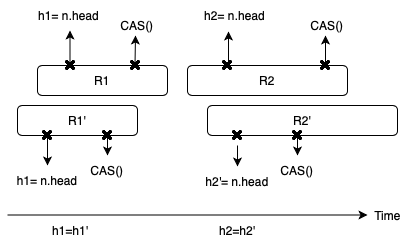
\includegraphics[width=3in]{pics/doublyrefresh.drawio.png}
  \caption{$R_2^\prime$'s \texttt{CAS} is executed after \texttt{h1=n.head}.}
\end{figure}



  Block \texttt{new} is created of new established subblocks of children of \texttt{n}(Lemma \ref{lem::createBlock}, Line 46). If \texttt{CAS} in Line 48 succeeds then by Lemma~\ref{lem::trueRefresh} new established blocks will be in \texttt{n}.
  
\begin{lemma}[Double Refresh] \label{doublyRefresh}
All operations in \texttt{n}'s children's blocks before line \texttt{35} are guaranteed to be in \texttt{n}'s blocks after Line~\texttt{37}.
\end{lemma}
\begin{proof}
Suppose block \texttt{b} with index \texttt{i} is in the the left child of \texttt{n} before the line 35. By Lemma~\ref{head} it follows that \texttt{n.left.head} is greater than \texttt{i}. \texttt{Refresh()} calls \texttt{CreateBlock()} and creates a block from blocks between \texttt{n.blocks[n.head].end\textsubscript{left}} and \texttt{n.left.head} in the left child, which contains \texttt{b} as well. First it tries to append it in \texttt{n.blocks.head} and if it was succsuful it continues recursivley. If not it tries again, and if the second call of \texttt{Refresh()} in Line 36 fails. It means there is another \texttt{Refresh} which has reah its \texttt{i} after the Line 35, so it contains \texttt{b} as well.
\end{proof}
\texttt{CreateBlock()} reads blocks in the children that do not exist in the parent and aggregates them into one block. If a \texttt{Refresh()} procedure returns true it means it has appended the block created by \texttt{CreateBlock()} into the parent node's sequence. So suppose two \texttt{Refresh}es fail. Since the first \texttt{Refresh()} was not successful, it means another CAS operation by a \texttt{Refresh}, concurrent to the first \texttt{Refresh()}, was successful before the second \texttt{Refresh()}. So it means the second failed \texttt{Refresh} is concurrent with a successful \texttt{Refresh()} that assuredly has read block before the mentioned line \texttt{35}. After all it means if any of the \texttt{Refresh()} attempts were successful the claim is true, and also if both fail the mentioned claim still holds.

\begin{lemma}[Append]\label{append}
 When \text{\texttt{Append(op)}} is finished, \texttt{op} appears exactly once in a block of \texttt{root.blocks}.
\end{lemma}
\begin{proof}
\texttt{Append(op)} adds \texttt{op} to \texttt{l\textsubscript{p}.blocks}(Line~\ref{addOP}) and \texttt{Propagate()} recursively propagates \texttt{op} up to the root.
By lemma \ref{doublyRefresh} we know that operation \texttt{op} propagates from child to parent at each level.
\end{proof}

\begin{lemma}[Block Size Upper Bound]\label{blockSize}
Each block in a node contains at most one operation from each processs.  
\end{lemma}
\begin{proof}
  Note that \texttt{prevIndex} and \texttt{lastIndex} defined in lines \ref{lastLine}, \ref{prevLine} are the indices defined in the Definition~\ref{def::subblock}. After a block has propagated to the parent the blocks between \texttt{prevIndex} and \texttt{lastIndex} make up to the parent (Lemma~\ref{doublyRefresh}). The number of new operations which have not propagated yet to the parent cannot be more than $p$. If so by the law of pigeonholes there is a process which has appended two concurrent operations.
\end{proof}

\begin{lemma}[Subblocks Upperbound]\label{subBlocksBound}
Each block in a node  has at most $p$ subblocks.
\end{lemma}
\begin{proof}
  From Line~\ref{addOP} it is induced directly that each block contains at least one operation. Now it follows directly by Lemma \ref{blockSize}.
\end{proof}

\begin{definition} [Ordering of operations inside a node] \label{ordering}
$\blacktriangleright$ Note that from Lemma \ref{blockSize} we know there is at most one operation from each process in a given block.

\begin{itemize}
  \item $E(n,i)$ is the sequence of enqueue operations that are member of \texttt{n.blocks[i]} ordered by process id.
  \item 
$D(n,i)$ is the sequence of dequeue operations that are member of \texttt{n.blocks[i]} ordered by process id.
\item $D(n)=D(n,1).D(n,2).D(n,3)...$
\item $L=E(root,1).D(root,1).E(root,2).D(root,2).E(root,3).D(root,3)...$
\end{itemize}
\end{definition}

\begin{theorem}
The queue implementation is linearizable.
\end{theorem}
\begin{proof}
  We show that the ordering $L$ stored in the root, satisfies the properties of a linearizable ordering.
  \begin{enumerate}
    \item If $op_1$ ends before $op_2$ begins in $E$, then $op_1$ comes before $op_2$ in $T$.\\$\blacktriangleright$ This is followed by Lemma \ref{append}. The time $op_1$ ends it is in root, before $op_2$, by Definition \ref{ordering} $op_1$ is before $op_2$.
    \item Responses to operations in $E$ are same as they would be if done sequentially in order of $L$. \\$\blacktriangleright$ Enqueue operations do not have any response so it does no matter how they are ordered. It remains to prove  Dequeue $d$ returns the correct response according to the linearization order. By Lemma \ref{computeHead} it is deduced that the head of the queue at time of the linearization of $d$ is computed properly. If the Queue is not empty by Lemma \ref{get} we know that the returning response is the computed index element.
  \end{enumerate} 
\end{proof}

\begin{lemma}[Get] \label{get}
\texttt{Get(n,b,i)} returns $i$th Enqueue in $E(n,b)$.
\end{lemma}
\begin{proof}
It is obvious that \texttt{Get(leaf l,b,1)} returns the operations stored in $b$th block of leaf $l$. To find the \texttt{i}th enqueue in block \texttt{b} of an internal node \texttt{n} in line 87 it is decided that it resides in the left child or the right child. This decision is made by Definition of $E(n,b)$. After that Lines 88, 92 search the proper subblocks of \texttt{b}. From Definition~\ref{def::subblock} weknow the subblocks of the $b$th block are within the \texttt{prevBlock} and \texttt{lastBlock} block of the \texttt{CreateBlock()}.
\end{proof}

\begin{lemma}[Index]
 Index(n,b,i) returns the rank in the $D(root)$ of ith Dequeue in $D(n,b)$.
\end{lemma}
\begin{proof}
  \texttt{Index(n,b,i)} computes superblock of $i$th Dequeue in $b$th block of \texttt{n} in \texttt{n.parent} and then computes the order in $D(n.parent, superblock)$. Then calls \texttt{index()} on \texttt{n.parent} recursively. It is easy to see why the second is correct. Correctness of computing superblock comes from Lemma \ref{superBlock}.
\end{proof}

\begin{lemma}[Computing SuperBlock]\label{superBlock}
  If \texttt{Index(n,b,i)} performs line 101, then \texttt{superblock} contains \texttt{i}th Dequeue in \texttt{b}th block of node \texttt{n}.
\end{lemma}
\begin{proof}
\begin{enumerate}
 \item Value read for \texttt{super[b.time]} in line 101 is not null.\\$\blacktriangleright$
  Values \texttt{c\textsubscript{dir}} read in lines 23, \texttt{super} are set before incrementing in lines 26,27.

 \item \texttt{super[]} preserves order from child to parent; if in a child block \texttt{b} is before \texttt{c} then \texttt{b.time} $\leq$ \texttt{c.time} and \texttt{super[b.time]} $\leq$ \texttt{super[c.time]}\\$\blacktriangleright$
  Follows from the order of lines 60, 48, 49.

% \item In a propagate step at most 2 different time values are read \\ If there are more than 2 numbers then the smallest number should have been propagated far before.
% \item There are at most $p^2$ blocks with same time value in a node. \\ At most p processes could die before line 27 and each contains at most p elements.
 \item \texttt{super[i+1]-super[i]}$\leq p$
\\$\blacktriangleright$
 In a Refresh with successful CAS in line 46, \texttt{super} and \texttt{counter} are set for each child in lines 48,49. Assume the current value of the counter in node \texttt{n} is \texttt{i+1} and still \texttt{super[i+1]} is not set. If an instance of successful \texttt{Refresh(n)} finishes \texttt{super[i+1]} is set a new value and a block is added after \texttt{n.parent[sup[i]]}. There could be at most $p$ successful unfinished concurrent instances of \texttt{Refresh()} that have not reached line 49. So the distance between \texttt{super[i+1]} and \texttt{super[i]} is less than $p$.

 \item Superblock of \texttt{b} is within range $\pm 2p$ of the \texttt{super[b.time]}.
\\$\blacktriangleright$
\texttt{super[i]} is the index of the superblock of a block containing block b, followed by Lemma \ref{superCounter}. It is trivial to see that \texttt{n.super} and \texttt{n.b.counter} are increasing. \texttt{super(b)} is the real superblock of b. \texttt{super(t]} is the index of the superblock of the last block with time \texttt{t}. If \texttt{b.time} is \texttt{t} we have:
$$super[t]-p\leq super[t-1]\leq super(t-1] \leq super(b) \leq super(t+1)\leq super(t+1]\leq super[t]+p$$

\end{enumerate}
\end{proof}

\begin{lemma}[Computing Queue's Head] \label{computeHead}
  Let Q be state of the queue if the operations before ith Dequeue in $L(root)$ are applied on the Queue sequentially and X be the head of Q. If Q is empty \texttt{ComputeHead(i,b)} returns -1, otherwise
 returns index in $E(root,b)$ of X.
  \end{lemma}

\begin{lemma}[Validity of \texttt{head}]\label{head}
No two blocks are written in the same index in \texttt{n.blocks}.
\end{lemma}
\begin{proof}
  \texttt{head} is incremented in lines 51, 54 after trying to append a block to the index of the last \texttt{head} read. If it was successful, we have to do this, but if it was unsuccessful, it means it has appended to the index before, so we have to update the \texttt{head}. If a process dies before line 51, another process will increment \texttt{head} in line 54.
\end{proof} 

\begin{lemma}[Validity of \texttt{super} and \texttt{counter}]\label{superCounter}
If \texttt{super[i] $\neq$ null}, then \texttt{super[i]} in node \texttt{n} is the superblock of a block with \texttt{time=i}.
\end{lemma}
\begin{proof}
After a successful CAS in line 46 \texttt{super} and \texttt{counter} are modified in both children. \texttt{super[i]} is supposed to be the superblock of a block with \texttt{time}=i and \texttt{counter} is the timer in each node. \texttt{super[i]} and \texttt{counter=i} are expected to update after a bunch of blocks with \texttt{time=i} have been aggregated together into a block in the parent. If the process dies before line 48 these values remain unchanged and incoming blocks will get the same \texttt{time}. We claim that our algorithm still works since at most $p$ processes die and it will not change our complexity. If a process dies right after line 48, then \texttt{counter} will remain the same and \texttt{super[i]} is correct. Furthermore we are sure that when \texttt{super[i]} is read it will not be \texttt{null}.
\end{proof}

\begin{lemma}[Search Ranges]\label{search}
  Preconditions of all invocation of \texttt{BSearch} are satisfied.
\end{lemma}
\begin{proof}
  
Line 83: \texttt{Get(i)} is called if the result of a dequeue is not null. The search is among all blocks in the root.

Line 88: This search tries to find the ith enqueue, knowing that it is in the left child. Search is done over the left subblocks. The start and end of the range are followed by definition. Line 92 is the same.

Line 101: Here, the goal is to find the superblock. We know the distance between answer and the \texttt{super[i]} is at most $p$, since at most $p$ processes could die.

\end{proof}

\paragraph{Overall}

The main difference between the main algorithm and the block tree is that we separate enqueues and dequeues, compute the number of non-null dequeues and the Queue's size in each block in the root. We emphasize that these changes work correctly; every other claim in Block trees applies here.

















\section{Make first level search fast}
\begin{algorithm}
\caption{Modified Queue \label{algQx}}
\begin{algorithmic}[1]
\begin{multicols}{2}

%\Statex \textbf{Structure}

%\Statex $\blacktriangleright$ \texttt{extends Queue Algorithm}


%\Statex $\blacktriangleright$\texttt{\textsl{RBTNode} RBTRoot}  \Statex
%  \textsf{pointer to an RBTNode, that is root of the RBTree}


\Statex $\blacktriangleright$ \texttt{\textsl{PRBTree[RBTNode]} rootBlocks}
  \Statex \textsf{A persistant redblack tree supporting \texttt{append(n),get(i),split(j)}}. \texttt{append(n)} returns \texttt{true} in case successful.


\Statex $\blacktriangleright$ \texttt{\textsl{RBTNode}}
\begin{itemize}

  \item \texttt{\textsl{RootBlock} block}



  \item \texttt{\textsl{int} age}
  
  \textsf{number of finished operations in the block}

  \item \texttt{\textsl{int} step}
  
  \textsf{If this node is the root of the RBTree, then step shows the number of appended nodes to the RBTree}

  
%  \item \texttt{some RBTRee attributes like left,right children}

\end{itemize}


\Statex $\blacktriangleright$ \texttt{\textsl{leaf} extends Node}
\begin{itemize}
  \item \texttt{\textsl{int[]} response}
  
  \textsf{leaf.response[i] stores response of leaf.ops[i]}
  
  \item \texttt{\textsl{int} maxOld}

  \textsf{Index of the youngest old block in the root that this process has seen yet.}
  
\end{itemize}

%\Statex $\blacktriangleright$ \texttt{\textsl{RBT(RBTnode n)}}
%  \Statex \textsf{Gives us RBTree  persistentoperations if n is root of a RBTRee, for example RBT(n).append(x) appends x if to the redblack tree with n as root. A persistent append is an append which only contains the changed nodes.}

\Statex



\Function{boolean}{Refresh}{\textsl{node} n} \Comment if n is root
\State \texttt{new=CreateBlock()} \Comment TODO
\If{\texttt{new.num==0}} \Return{\texttt{true}}
\ElsIf{\Call{RBTAppend}{new}}
\Statex..\EndIf
\EndFunction{Refresh}

\Statex

\Function{<int, int>}{Index}{\textsl{node} n, \textsl{int} b, \textsl{int} i} \Comment{Returns the order in the root among dequeus, of ith dequeue in bth block of node n}
\If{\texttt{n {\keywordfont is} root}} \Return \texttt{search in the current RBTRee}
\Else
..
\EndIf
\EndFunction{Index}

\Statex

\Function{Object}{Dequeue()}{}
\State ..
\State \texttt{N\textsubscript{i}= RBTnode n that n.block contains the invocation of Dequeue}
\State \texttt{N\textsubscript{r}= RBTnode n that n.block contains the response of Dequeue}
\State \texttt{N\textsubscript{i}.age= N\textsubscript{i}.age+1} \Comment{this is a shared counter}
\State \texttt{N\textsubscript{r}.age= N\textsubscript{r}.age+1}
\If{\texttt{N\textsubscript{i} or N\textsubscript{r} become old}} \texttt{update maxOld}
\EndIf
\EndFunction{Dequeue}


\pagebreak
%\Function{void}{Update(Root Block B)}{}
%\If{\texttt{B.todo==0}}
%\If{\texttt{B.left.old-subtree} and \texttt{B.right.old-subtree}}
%\State \texttt{B.old-subtree= True}
%\If{\texttt{B.parent!=root}}
%\State \texttt{Update(B.parent)}
%\EndIf\EndIf
%\EndIf
%\EndFunction{Update}
%\Statex

\Function{void}{RBTAppend}{block b} \Comment{\textsf{adds block b to the \texttt{rootBlocks}}}
\State \texttt{root= rootBlocks.root}
\If{\texttt{root.step\%$p^2$==0}}
\State \texttt{Help()}
\State \texttt{CollectGarbage()}
\EndIf
\State \texttt{new= RBTnode(b,0,null)}
%\State \texttt{r= pointer to root of the RBT(h).append(n)}
%\State \texttt{*r.step= h.step+1}
%\State \texttt{RBTRoot.CAS(h,r)}
\State \Return \texttt{rootBlocks.append(new)}
\EndFunction{RBTAppend}
\Statex


\Function{void}{Help}{}\Comment{Helps pending operations}
\State{last= l.head-1}
\For{\texttt{leaf l in leaves}}
\If{\texttt{l.blocks[last] is not null}}
\If{op \textbf{is} DEQ}
\State\texttt{run \texttt{Dequeue()}  for \texttt{l.ops[last]} after Propagate()}
\State \texttt{write the response to l.responses[last]}
\EndIf
\EndIf
\EndFor
\EndFunction{Help}
\Statex

\Function{void}{CollectGrabage}{}\Comment{Collects the old root blocks.}
\State \texttt{l=FindYoungestOld(Root.Blocks.root)}
\State \texttt{t1,t2= RBT.split(l)}
\State \texttt{RBTRoot.CAS(t2.root)}
\EndFunction{CollectGrabage}

\Statex

\Function{Block}{FindYoungestOld}{b}
\State\Return  \texttt{read all maxOld values among leaves and decide the largest one} \Comment{There is no need to do a sasDK;Lnapgshot.}
\EndFunction{findYoungestOld}

\Statex

\Function{response}{FallBack}{op i}

\If{operation i in leaf l cannot find its desired RootBlock}

\State \Return \texttt{l.response[i]}
\EndIf

\EndFunction{FallBack}

\end{multicols}
\end{algorithmic}
\end{algorithm}


\bibliographystyle{abbrv}
\bibliography{main}

\end{document}






